\documentclass[11pt]{article}
\usepackage[margin=1.1in]{geometry}
\usepackage{amsmath,amssymb,amsthm}
\usepackage{booktabs}
\usepackage{array}
\usepackage{graphicx}
\usepackage[hidelinks]{hyperref}
\usepackage[expansion=false]{microtype}
\usepackage[authoryear,round]{natbib}
\usepackage{setspace}
\onehalfspacing

\theoremstyle{plain}
\newtheorem{proposition}{Proposition}
\newtheorem{lemma}{Lemma}
\newtheorem{corollary}{Corollary}
\theoremstyle{definition}
\newtheorem{definition}{Definition}
\newtheorem{assumption}{Assumption}
\theoremstyle{remark}
\newtheorem{remark}{Remark}

\newcommand{\Lam}{\Lambda}
\newcommand{\WL}{W_{\!L}}
\newcommand{\Sh}{\bar s}
\newcommand{\Delt}{\Delta}
\newcommand{\ebar}{\underline{e}}
\newcommand{\mbar}{\underline{m}}
\newcommand{\lbar}{\bar\lambda}

\title{Nested Races: Laboratory Enforcement and the Strategic Form of\\ Interstate Restraint in the AGI Competition}
\author{Emile Naude\thanks{Lleverage; MSc Finance \& Economics, Barcelona School of Economics (Universitat Pompeu Fabra / Universitat Autònoma de Barcelona). Replication code for all numerical results accompanies the paper. A statement on the use of AI tools appears in the acknowledgements. All errors are the author's.}}
\date{September 2026}

\begin{document}
\maketitle

\begin{abstract}
\noindent This article models interstate competition over advanced artificial intelligence as the continuation of a laboratory safety contest under imperfectly implemented regulation. States choose regulatory intensity; effective regulation depends on monitoring; laboratories choose safety in a winner-take-most contest while internalising only part of a shared catastrophe; interstate payoffs are laboratory continuation values. A derived identity links the ordering of states' incentives to regulate to the catastrophe risk generated by unilateral and mutual restraint. Under linear average risk and the baseline contest, laboratory responses rule out a Stag Hunt; over the illustrated parameter range, as perceived catastrophe intensity rises the game passes from a Prisoner's Dilemma through Chicken to dominant restraint. A weakest-link risk aggregation rule, or laboratories that cut safety when they fall behind, generate assurance regions in the examples examined. The analysis therefore identifies assumptions about risk and domestic implementation that must be established before prescribing either reassurance or burden-sharing. Monitoring shifts these incentives through enforcement, alongside liability and sanction intensity, and regulation announced below an enforcement threshold changes laboratory behaviour not at all. Policy conclusions are conditional on the laboratory responses and parameter ranges analysed.

\medskip\noindent\textbf{Keywords:} artificial intelligence governance; two-level games; arms control; verification; contests; risk aggregation; Chicken; Stag Hunt; nested games

\noindent\textbf{JEL codes:} C72; D74; D62; F51; L51; O33

\noindent\textit{Version 1.1, 16 September 2026. Working paper; comments welcome.} \textit{Correspondence:} \texttt{naudemile@gmail.com}. \textit{ORCID:} 0009-0006-4950-7621.
\end{abstract}

\section{Introduction}

In 2023 and 2024, leading governments issued declarations of restraint concerning frontier artificial intelligence: an intergovernmental declaration on frontier-model risk \citep{bletchley2023}, voluntary commitments by developers brokered by the White House \citep{whitehouse2023}, reporting thresholds for large training runs \citep{eo14110}, and in the European Union a statutory regime \citep{euaiact2024}. Throughout, the compute devoted to frontier training runs continued its multi-year growth \citep{sevilla2022,sastry2024}, evaluation gates were adopted by the laboratories themselves and remained self-reported, and no cross-border mechanism for verifying what a foreign laboratory was training was established \citep{wasil2024}. Then the rhetoric turned. In January 2025 the United States revoked its reporting order \citep{eo14148}, directed that measures taken under it be reviewed and removed \citep{eo14179}, and by mid-year had adopted acceleration as national policy \citep{aiactionplan2025}; the 2025 summit cycle dropped safety from its title. Announced restraint at the level of states first coexisted with continued racing at the level of firms, then gave way to it.

On 12 September 2026 the chief executive of one frontier laboratory published a proposal to slow the pace of capability improvement, citing an industry-wide acceleration driven by models building their successors and an incident in which a swarm of agents attacked targets they had not been asked to attack \citep{amodei2026}. The proposal, referred to below as the pacing proposal, has three steps: permanent third-party evaluators embedded inside laboratories, which the author's own laboratory adopted unilaterally; coordination among democratic-country laboratories, with government cover on antitrust; and agreements with authoritarian governments subject to verification. It ties any slowdown to the size of the lead democracies hold, which export controls, anti-distillation enforcement, and weight security are to protect. Whether a leading laboratory's unilateral move on verification but not on speed, and a slowdown bounded by its lead, are rational strategies is a question a model of nested races should be able to answer. Corollary~1 and Appendix~C address it.

Standard treatments of the AGI race cannot describe this pattern because they model only one level. One family treats the leading states as players in a Prisoner's Dilemma (PD), so that unilateral restraint is dominated and racing is inevitable.\footnote{Policy-adjacent statements include \citet{abraham2025}, who derive both a PD region and a coordination region, and \citet{katzke2025}, who argue that the race is self-defeating.} Another treats the same interaction as an assurance game: once catastrophe risk is taken seriously, mutual restraint is also an equilibrium and the problem is trust rather than dominance \citep{katzke2025,roussel2026}. Both families write interstate payoffs directly. Neither asks whether the laboratories that implement a state's choice will in fact behave as the payoff matrix assumes, or how the answer depends on what the state can observe.

This article treats the AGI competition as a nested game in Putnam's sense \citep{putnam1988} and in Tsebelis's \citep{tsebelis1990}: the interstate game is played over payoffs that are themselves the equilibrium outcomes of a domestic game. At Level~I two states choose regulatory intensity. At Level~II frontier laboratories choose safety effort in a winner-take-most contest, internalising only a fraction of a shared catastrophe. Monitoring precision determines how much of an announced regulation reaches the laboratory. The organising claim is that \emph{whether states can sustain restraint in an AI race depends on how domestic enforcement changes both laboratory safety and the gains from unilateral acceleration}. Three results follow from writing the model this way rather than positing interstate payoffs.

First, the laboratory stage has a precipice structure: when the laboratory's internalised share of catastrophe is below an explicit threshold, the competitive return to speed dominates and safety effort collapses to a corner. Announced regulation changes this only when effective sanctions exceed a ``bite'' threshold, and it implements the regulator's target only above a second, higher threshold that need not lie in the feasible range. Perfect monitoring can be insufficient; the required enforcement depends on liability, sanction intensity, and the size of the prize.

Second, and centrally, the strategic form of the interstate game is determined, not chosen. Let $D_R$ be a state's gain from regulating when its rival regulates and $D_A$ its gain from regulating when its rival accelerates. A one-line identity shows that $D_R-D_A=(W/2+\Lam\ell)\,\Delt$, where $\Delt$ compares catastrophe risk under unilateral restraint with the average of risk under mutual restraint and mutual racing, and each of these is a laboratory-equilibrium object. A Stag Hunt requires $D_R>0>D_A$ and hence $\Delt>0$; Chicken requires $\Delt<0$. The sign of $\Delt$ orders the incentives; the levels of $D_R$ and $D_A$ determine whether the game exhibits dominance, Chicken, or a Stag Hunt. Two risk aggregation rules are analysed side by side. Under \emph{average risk}---catastrophe probability falls with mean safety across laboratories---$\Delt\le0$ is a theorem: the regulated laboratory facing an unregulated rival is discouraged and invests \emph{more} in safety, so unilateral restraint is less risky than the average of the symmetric profiles, and a Stag Hunt is excluded; in the illustration the game passes, as perceived catastrophe intensity rises, from a PD through a Chicken region into dominant restraint. Under \emph{weakest-link risk}---catastrophe probability is set by the least safe laboratory, so that one racing laboratory keeps risk high---$\Delt>0$ in every case computed and the middle region is a Stag Hunt. A third route to the assurance game runs through behaviour rather than the aggregation rule: if laboratories respond to falling behind by cutting safety, the pattern \citet{fernandez2026} document experimentally, a Stag Hunt emerges even under average risk. Which aggregation rule fits advanced AI is open---the weakest-link case is natural if catastrophe comes from whichever laboratory first crosses a capability threshold unsafely, the average case if risk accumulates across deployed systems---and the article argues that this, together with how laboratories respond to relative position, is the question on which the PD-versus-trust-dilemma debate actually turns. Section~6 also maps the two camps of the policy debate onto the model's parameters. Those who expect the first mover to gain durable hegemony hold a high prize-to-loss ratio and, typically, a low catastrophe probability; those who expect a temporary lead and a serious chance of loss of control hold the reverse. The two camps sit in different regions of the same game, and the model says which instruments each region calls for.

Third, monitoring precision moves the thresholds between regions. At parameter values where regulation does not change laboratory behaviour, it adds only its implementation cost, so mutual acceleration is dominant whatever the perceived risk. As monitoring improves, the loss at which restraint becomes dominant falls roughly fivefold in the numerical illustration. Verification is not a side condition on an otherwise fixed game; it shifts which game is being played.

The contribution is the connection from domestic implementation and laboratory responses to interstate strategic structure. It is not the discovery that AI races can involve coordination \citep{abraham2025}, nor the first introduction of monitoring into AI-race incentives \citep{bova2023}; the laboratory precipice is inherited from \citet{armstrong2016}, and the observation that a large shared loss can flip incentives toward restraint is classical security-dilemma theory \citep{jervis1978,snyder1971}. The model is static and complete-information. It does not formalise Putnam's ratification win-sets or the security cost of intrusive monitoring identified by \citet{coe2020}; those ideas motivate the treatment of monitoring precision as a scarce parameter but are not derived.

Section~2 situates the argument. Section~3 sets out the model. Section~4 solves the laboratory stage. Section~5 derives the interstate game from laboratory continuation values. Section~6 gives a numerical illustration. Section~7 discusses verification, observable implications, what would have to be measured to identify the game, and limits. Section~8 asks what laboratories' own calls for regulation are consistent with. Section~9 draws bounded policy conclusions. Proofs are in Appendix~A, the numerical procedure in Appendix~B, and three extensions---a capability lead treated as a stock, divisible restraint, and asymmetric enforcement across the two states---in Appendices~C, D, and~E.

\section{Related work}

\paragraph{Laboratory races.} \citet{armstrong2016} model AI development as a race in which competitive pressure erodes safety. Evolutionary treatments extend the logic to population dynamics and network structure \citep{han2020,cimpeanu2022}. International technology-race models study safety--performance tradeoffs under shared disaster risk: \citet{stafford2022} on corner-cutting by laggards and risk compensation; \citet{emery2024} on how private and public information about relative capability affects disaster risk in decisive races. The last is the closest published benchmark for the present article's method---mechanisms are followed through a specified model to their implications---and the present article's potential distinction is domestic delegation: the state does not race, its laboratory does. \citet{tan2025} analyses continuous-time preemption with shared catastrophe and shows that symmetric ruin costs can cancel in the equilibrium indifference condition; nesting shows that shared loss does not cancel in the principal--agent wedge between states and laboratories.

\paragraph{Regulators and firms.} \citet{bova2023} model regulators, AI firms, detection, enforcement, and conditional compliance in an evolutionary framework, including risk-dominance thresholds. That work already establishes that enforcement quality governs whether regulation induces safe development; the present article does not claim priority for that mechanism. What it adds is the upper tier: the regulator's own choice is embedded in an interstate game whose payoffs depend on the enforcement outcome. Contest-theoretic treatments of dangerous-technology development \citep{naude2020,polborn2025,bdm2026} analyse entry, safety--speed allocation, market structure, and public intervention in a single layer; their competitor-count results, which need not follow the usual ``more racers, more danger'' intuition, are consistent with the conditional comparative static derived in Section~4.

\paragraph{Interstate framings.} \citet{abraham2025} model U.S.--China competition and derive both a PD region and a coordination region depending on beliefs about risk. \citet{katzke2025} and \citet{roussel2026} argue that sufficiently high perceived loss of control makes restraint or a moratorium self-interested. Nesting endorses the threshold logic and adds two qualifications: interstate restraint moves laboratory safety only above a monitoring threshold, and the coordination region that appears once restraint is an equilibrium is a Stag Hunt only under a particular risk aggregation rule; under the baseline it is Chicken. \citet{hendrycks2025} discuss deterrence-by-sabotage postures; in the present framework such postures alter continuation values after acceleration and are an extension.

\paragraph{Two-level games, assurance, and arms control.} \citet{putnam1988} and \citet{tsebelis1990} supply the nesting logic; \citet{evans1993} and \citet{milner1997} develop its domestic side; \citet{downs1996} caution that observed compliance may reflect shallow commitments, a point that bears directly on self-reported safety. \citet{jervis1978}, \citet{snyder1971}, and \citet{glaser1997} explain when conflict has PD, Chicken, or Stag Hunt structure; the present article derives which of these obtains from primitives rather than assigning it. \citet{schelling1960,schelling1966} and \citet{kydd2000,kydd2005} supply the vocabulary of commitment and reassurance that applies once a coordination problem has been shown to exist. \citet{coe2020} argue that arms control is rare because monitoring must be revealing enough to detect cheating without threatening the monitored state's security. Verification of training is now a literature of its own: compute-based verification of training rules \citep{shavit2023}, lessons from nuclear verification \citep{baker2023}, taxonomies of verification methods and evasion \citep{wasil2024,scher2024}, and compute governance more broadly \citep{sastry2024,brundage2020}. These give the parameter $m$ a concrete interpretation. \citet{hirshleifer1983} on weakest-link public goods and \citet{vanhuyck1990} on minimum-effort coordination supply the intuition behind the risk-aggregation-rule result in Section~5.

\paragraph{Behavioural evidence.} \citet{fernandez2026} report an experiment in which unsafe choices track relative race position: falling behind increases unsafe play. Section~5 shows that this response, if it characterises frontier laboratories, is one of two conditions under which the interstate game can be an assurance game at all.

\section{The model}

\subsection{Players, timing, information}

There are two states, $i\in\{U,C\}$, each with one frontier laboratory; Section~4.3 extends the laboratory stage to $n$ laboratories. All players are expected-utility maximisers and all primitives are common knowledge.

\begin{enumerate}
\item \emph{Regulation.} States simultaneously choose $r_i\in\{0,1\}$: $r_i=0$ is Accelerate ($A$), $r_i=1$ is Regulate ($R$).\footnote{Continuous $r_i\in[0,1]$ changes nothing in the laboratory stage, where only effective regulation matters; the binary restriction is used because the interstate results concern the strategic form of a $2\times2$ game.}
\item \emph{Monitoring.} Effective regulation in jurisdiction $i$ is $e_i=m\,r_i$, where $m\in[0,1]$ is monitoring precision, a technological and institutional parameter common to both states. Section~7.1 decomposes $m$ into inspectability, detection, and leakage.
\item \emph{Safety.} State choices are publicly observed. Each laboratory then observes $(e_U,e_C)$ and chooses safety effort $s_j\in[0,1]$ simultaneously.
\item Payoffs realise.
\end{enumerate}

\subsection{Primitives}

\emph{Contest.} Laboratory $j$'s speed is $x_j=1-s_j+\varepsilon$ with $\varepsilon>0$: safety slows development but does not halt it. The probability that $j$ first achieves controllable strategic advantage is the Tullock ratio
\begin{equation}
\pi_j(s)=\frac{x_j}{X}, \qquad X:=x_j+x_k .
\label{eq:contest}
\end{equation}
The floor $\varepsilon$ keeps $\pi_j$ continuous on $[0,1]^2$; without it the contest is undefined when both laboratories choose $s=1$, and existence arguments fail. The two laboratories are assumed symmetric in capability: at equal caution they move at equal speed. Differences in compute and talent are treated as a lead that can be spent or eroded (Appendix~C) rather than as a permanent difference in speed, because access to chips, distillation of frontier models, and theft of weights make a flow advantage transient; Section~7.5 records what survives of the main identity when the assumption is dropped.

\emph{Catastrophe risk.} Three specifications of perceived catastrophe probability are analysed---three \emph{risk aggregation rules}, in the sense in which public-goods economics speaks of aggregation technologies \citep{hirshleifer1983}---treated as hypotheses about the world rather than as a baseline and alternatives. Which rule holds is not obvious and is not settled: it corresponds to the distinction between accumulative and decisive existential risk drawn by \citet{kasirzadeh2025}, and the literature has assumed one or the other without stating which. Under \emph{average risk},
\begin{equation}
Q^{\mathrm{A}}(s)=q_0\bigl(1-\alpha\,\Sh\bigr),\qquad \Sh=\tfrac12(s_U+s_C),\quad q_0\in(0,1),\ \alpha\in(0,1),
\label{eq:risk}
\end{equation}
so that each laboratory's safety reduces global risk by the same amount whatever the other does, as when harm accumulates across many deployed systems. Under \emph{weakest-link risk}, catastrophe probability is set by the least safe laboratory. To keep payoffs smooth the minimum is replaced by a normalised soft minimum,
\begin{equation}
Q^{\mathrm{W}}(s)=q_0\bigl(1-\alpha\,S_\tau(s)\bigr),\qquad S_\tau(s)=-\tau\log\!\Bigl(\tfrac12\bigl(e^{-s_U/\tau}+e^{-s_C/\tau}\bigr)\Bigr),
\label{eq:wl}
\end{equation}
which equals $s$ at any symmetric profile $(s,s)$ and converges to $\min\{s_U,s_C\}$ as $\tau\downarrow0$; the illustration uses $\tau=0.05$. This is the smooth analogue of the weakest-link public good of \citet{hirshleifer1983}, and it is the rule under which one racing laboratory keeps global risk high. The third specification, \emph{leader-link risk}, is introduced in Section~5.4 for a fast, discontinuous takeoff. In all three cases $Q$ is strictly positive and smooth. Sections~5.3--5.4 show that the strategic form of the interstate game differs across them, and Section~7 discusses how they could be distinguished empirically.\footnote{A fourth specification, $Q=q_0(1-\alpha\Sh^{\gamma})$ with $\gamma>1$, depends only on mean safety and therefore assigns the same risk to $(1,0)$ and $(0.5,0.5)$; it represents increasing returns to aggregate safety, not a weakest link. It is treated as a remark in Section~5.4.}

\emph{Laboratory payoff.} The prize $\WL>0$ is the laboratory's stake in the geopolitical/commercial prize $W$, $\WL=\sigma W$ with $\sigma\in(0,1]$. Catastrophe destroys the prize for everyone, so the prize is earned only with probability $1-Q$; this is imposed consistently at both levels. Laboratories internalise a fraction $\lambda\in[0,1]$ of the shared catastrophe loss $\ell>0$ (liability, reputation, expected future licensing). Safety costs $\kappa s_j^2/2$. Expected sanctions for low measured safety are $\rho\,e_j(1-s_j)$, $\rho\ge0$:
\begin{equation}
u_j=(1-Q)\,\pi_j\,\WL-\tfrac{\kappa}{2}s_j^2-\lambda\,Q\,\ell-\rho\,e_j\,(1-s_j).
\label{eq:lab}
\end{equation}
The sanction term is the channel through which effective regulation reaches laboratory incentives; without it $e_i$ would be irrelevant to laboratory behaviour. The term is a reduced form for a monitor that observes safety with noise and penalises measured unsafety: if the penalty is linear in the measurement and the laboratory is risk-neutral, measurement noise cancels in expectation and $m$ is the probability that a violation is observed and attributed. Threshold or licence-revocation sanctions, under which false positives and negatives matter, are an extension (Section~7.1).

\emph{State payoff.} State $i$ internalises a fraction $\Lam\in(0,1]$ of the catastrophe loss and bears a direct cost $d\ge0$ of regulating (administrative, competitiveness, political):
\begin{equation}
V_i=(1-Q)\,\pi_i\,W-\Lam\,Q\,\ell-d\,r_i .
\label{eq:state}
\end{equation}
The state's probability of capturing the prize is its laboratory's contest probability; with one laboratory per state, $P_i=\pi_i$. The delay cost of regulation is endogenous---a regulated laboratory is slower, so $\pi_i$ falls---and $d$ captures only costs outside the contest.

\subsection{Nesting}

\begin{definition}[Nesting]
For each profile $r=(r_U,r_C)$ and monitoring precision $m$, the laboratories play the subgame $\Gamma^{\mathrm{lab}}(r,m)$ with payoffs~\eqref{eq:lab} evaluated at $e_i=mr_i$. Let $s^*(r,m)$ be its Nash equilibrium. State $i$'s payoff from $r$ is the continuation value $V_i(r,m)$ obtained by substituting $s^*(r,m)$ into~\eqref{eq:state}. The interstate game is the $2\times2$ normal form with these payoffs, and its equilibria together with $s^*$ constitute the subgame-perfect equilibria of the two-level game.
\end{definition}

The definition is the formal content of ``nested races''. Its discipline is that no interstate cell may be written independently of laboratory play. Section~5 shows that this discipline has teeth: it excludes strategic forms that single-layer treatments assume.

\section{The laboratory stage}

\subsection{Existence, uniqueness, and the first-order condition}

\begin{lemma}[Regularity]
Under average risk, $u_j$ is strictly concave in $s_j$ on $[0,1]$ for every $s_k$ and every $e_j$. A pure-strategy Nash equilibrium of $\Gamma^{\mathrm{lab}}$ exists for every $(e_U,e_C)$. When $e_U=e_C$, the symmetric equilibrium is unique.
\end{lemma}

Differentiating~\eqref{eq:lab} under average risk, with $\partial Q/\partial s_j=-q_0\alpha/2$ and $\partial\pi_j/\partial s_j=-x_k/X^2$ gives the marginal private return to safety,
\begin{equation}
\frac{\partial u_j}{\partial s_j}
=\frac{q_0\alpha}{2}\bigl(\pi_j\WL+\lambda\ell\bigr)-(1-Q)\frac{x_k}{X^2}\,\WL-\kappa s_j+\rho e_j .
\label{eq:foc}
\end{equation}
The first term is the value of protecting the prize and the internalised catastrophe loss; the second is the competitive cost of slowing down; the last two are cost and sanction. At a symmetric profile $s$ with $n$ laboratories, $\pi_j=1/n$ and $\partial\pi_j/\partial s_j=-(n-1)/(n^2(1-s+\varepsilon))$, so the symmetric first-order condition is
\begin{equation}
F(s;e,n):=\WL\!\left[\frac{q_0\alpha}{n^2}-\frac{(1-Q(s))(n-1)}{n^2(1-s+\varepsilon)}\right]-\kappa s+\frac{\lambda q_0\alpha\ell}{n}+\rho e=0,
\label{eq:symfoc}
\end{equation}
with $Q(s)=q_0(1-\alpha s)$. $F$ is defined for average risk; the other aggregation rules are analysed numerically. The factor $n^2$ in the contest derivative is the standard Tullock result that an individual contestant's marginal return to effort at a symmetric profile is $(n-1)/n^2$ times the prize \citep{tullock1980}. $F$ is strictly decreasing in $s$, which is what delivers uniqueness of the symmetric equilibrium.

\subsection{Precipice and implementation}

\begin{proposition}[Precipice]
Under average risk with $e_U=e_C=e$, the symmetric equilibrium is
\[
s^*(e)=\begin{cases}0,& F(0;e,n)\le0,\\ \text{the unique root of } F(\cdot;e,n)\text{ in }(0,1),& F(0;e,n)>0>F(1;e,n),\\ 1,& F(1;e,n)\ge0.\end{cases}
\]
The corner $s^*=0$ obtains if and only if
\begin{equation}
\lambda\le\lbar(e):=\frac{\dfrac{\WL}{n}\!\left[\dfrac{(1-q_0)(n-1)}{1+\varepsilon}-q_0\alpha\right]-n\rho e}{q_0\alpha\ell}.
\label{eq:lambdabar}
\end{equation}
$s^*(e)$ is weakly increasing in $e$, $\lambda$, $\rho$, and $\ell$, strictly so on the interior when the relevant coefficient is positive ($\lambda>0$ for $\ell$; $e>0$ for $\rho$), and weakly decreasing in $\WL$ whenever the bracket in~\eqref{eq:symfoc} is negative, i.e.\ whenever the competitive stake dominates the prize-protection motive.
\end{proposition}

The upper corner matters for the interstate results. Because $\lambda q_0\alpha\ell/n$ grows without bound in $\ell$, $F(1;0,n)>0$ for sufficiently large $\ell$: with $\lambda>0$, full safety becomes privately optimal even without regulation. All four regulatory profiles then coincide, regulation changes neither risk nor winning probabilities, and $D_R=D_A=-d$. The sequence results below are therefore stated on an interval of $\ell$, not for all $\ell$.

The threshold $\lbar(0)$ is positive exactly when the competitive stake exceeds the prize-protection motive, $(1-q_0)(n-1)/(1+\varepsilon)>q_0\alpha$: a laboratory that believes catastrophe is very likely protects its expected prize by slowing down even without liability. This is the continuous analogue of the precipice in \citet{armstrong2016}: for internalisation below $\lbar$, winner-take-most competition drives safety to the corner. The result is stated as an explicit threshold rather than as ``typically'', because whether laboratories skimp depends on liability, sanctions, and the curvature of the contest.

For implementation, fix $r=(1,1)$, so $e=m$, and let $n=2$. Define the regulator's target as the common safety level a state would choose for both laboratories if it could dictate it, counting its own laboratory's cost:
\begin{equation}
s^c:=\arg\max_{s\in[0,1]}\Bigl[(1-Q(s))\tfrac{W}{2}-\Lam Q(s)\ell-\tfrac{\kappa}{2}s^2\Bigr]
=\min\Bigl\{1,\ \frac{q_0\alpha\,(W/2+\Lam\ell)}{\kappa}\Bigr\}.
\label{eq:sc}
\end{equation}
With $n$ laboratories split equally between the states and each state counting its own laboratories' costs, the cost term is $n\kappa s^2/4$ and $s^c_n=\min\{1,\,2q_0\alpha(W/2+\Lam\ell)/(n\kappa)\}$, which reduces to~\eqref{eq:sc} at $n=2$; a planner counting all laboratories' costs would use a different objective, and the two should not be mixed.

\begin{proposition}[Two implementation thresholds]
Under average risk with $n=2$, $r=(1,1)$, $\rho>0$, let $B:=F(0;0,2)$. Then $s^*(m)=0$ if and only if $B+\rho m\le0$. If $B<0$ the bite threshold is $e_0:=-B/\rho$ and announced regulation has no effect on laboratory behaviour for $m\le e_0$; if $B\ge0$ there is positive safety already at $m=0$ and no such region. For a target $s^c\in(0,1]$ define the required monitoring
\begin{align}
m_{\mathrm{req}}&:=\max\Bigl\{0,\,-\frac{F(s^c;0,2)}{\rho}\Bigr\},\notag\\
-\frac{F(s^c;0,2)}{\rho}&=\frac{1}{\rho}\left\{\WL\!\left[\frac{(1-Q(s^c))}{4(1-s^c+\varepsilon)}-\frac{q_0\alpha}{4}\right]+\kappa s^c-\frac{\lambda q_0\alpha\ell}{2}\right\}.
\label{eq:ebar}
\end{align}
The target is attained if and only if $m\ge m_{\mathrm{req}}$, and is feasible within $m\in[0,1]$ if and only if $m_{\mathrm{req}}\le1$; if $s^c=0$ implementation is automatic. Where $m_{\mathrm{req}}$ is positive and uncapped, it is increasing in $s^c$ (hence in $\Lam$ and $W$) and in $\WL$, and decreasing in $\lambda$ and $\rho$.
\end{proposition}

Two features distinguish this statement from a binary binding/non-binding distinction. First, there are two thresholds, not one: below $e_0$ a Regulate announcement is pure cost; between $e_0$ and $m_{\mathrm{req}}$ it moves safety but not to the target. Second, the target may be infeasible. Capping the threshold at $\min\{1,m_{\mathrm{req}}\}$ would conceal this; when $m_{\mathrm{req}}>1$ the instrument that must move is $\rho$, $\lambda$, or $\WL$, not $m$. In~\eqref{eq:symfoc} liability and expected sanctions $\rho m r$ enter additively, so they are substitutes at the laboratory margin, while monitoring and sanction intensity enter multiplicatively: monitoring makes sanctions effective, and liability can implement a given safety target with less of both. The case for monitoring over liability, if there is one, rests on what rivals can observe, which the complete-information model cannot speak to (Section~7).

\begin{corollary}[Verification without sanction]
Suppose $r=0$ and monitoring precision rises from $m$ to $m'>m$. Then $e_i=m'r_i=0$ and laboratory safety is unchanged. Monitoring alone moves laboratory incentives only through $\lambda$: if published findings raise the reputational or legal cost of skimping from $\lambda$ to $\lambda'$, the effect on safety is that of the liability instrument, and the bite and target thresholds are those of~\eqref{eq:lambdabar} and~\eqref{eq:ebar} at $\lambda'$.
\end{corollary}

The corollary bears on proposals that begin with verification and defer sanctions. Embedded evaluators with the right to publish raise $m$ and, through publication, $\lambda$; they do not raise $e$ until a regulator attaches consequences to what they find.

\begin{remark}[Greater state internalisation raises the required enforcement]
Because $F$ is decreasing in $s$, $m_{\mathrm{req}}$ rises with $s^c$ where it is positive and uncapped, and $s^c$ rises with $\Lam$. The intuition is direct: a state that internalises more of the catastrophe wants safer laboratories and therefore needs stronger enforcement to get them.
\end{remark}

\subsection{Number of laboratories}

Treat $n$ as continuous in~\eqref{eq:symfoc} for the local statement; the discrete comparison $s^*(n+1)<s^*(n)$ holds if and only if $F(s^*(n);e,n+1)<0$.

\begin{proposition}[Competitor count]
Let $\gamma=1$ and let $s^*(n)$ be the interior symmetric equilibrium. Then $s^*$ is locally increasing in $n$ if and only if
\begin{equation}
\WL\left[\frac{(1-Q(s^*))(n-2)}{1-s^*+\varepsilon}-2q_0\alpha\right]>n\,\lambda\,q_0\alpha\ell .
\label{eq:ncond}
\end{equation}
In particular, safety falls when $n$ rises from a duopoly, and it falls for every $n$ if internalisation $\lambda\ell$ is large; but for large $n$ and small $\lambda$ safety rises with the number of laboratories.
\end{proposition}

The condition separates two effects that are often conflated. Adding a competitor dilutes each laboratory's internalised catastrophe stake ($\lambda q_0\alpha\ell/n$), which lowers safety; this is the \citet{armstrong2016} channel. But under a Tullock contest it also lowers each laboratory's marginal return to speed, $(n-1)/n^2$, once $n>2$, which raises safety---the rent-dissipation effect familiar from contest theory \citep{tullock1980}. Which dominates is an empirical matter, consistent with the competitor-count findings in \citet{polborn2025}. Aggregate risk, which depends on mean safety, inherits the same ambiguity. The result should be read as a qualification of the existing literature rather than a prediction for the frontier race: with entry gated by compute and talent, the number of laboratories in contention is two or three and is not the margin that moves. The empirically relevant margin is cheaper proximity to the frontier through distillation or diffusion of weights, which is an erosion of the leader's lead (Appendix~C) and a leakage of enforcement (Section~7.1), not an additional symmetric competitor.

\subsection{Strategic interaction between laboratories}

The results of Section~5 turn on how a laboratory responds to its rival's safety.

\begin{lemma}[Cross effects]
For $\gamma=1$ and $n=2$,
\begin{equation}
\frac{\partial^2 u_j}{\partial s_j\,\partial s_k}=\WL\,(x_j-x_k)\left[\frac{q_0\alpha}{2X^2}+\frac{1-Q}{X^3}\right].
\label{eq:cross}
\end{equation}
Safety choices are strategic complements for the faster laboratory and strategic substitutes for the slower one; at a symmetric profile they are independent to first order.
\end{lemma}

A laboratory that is behind in the race faces a lower marginal return to speed when its rival pulls further ahead---the discouragement effect of Tullock contests---and responds by investing more in safety. This is the opposite of the behavioural pattern in \citet{fernandez2026}, in which falling behind increases unsafe play. The difference matters for the interstate game.

\section{The interstate stage}

\subsection{Continuation values and an identity}

Write the row state's continuation values as $u_{RR}=V_i(1,1;m)$, $u_{AA}=V_i(0,0;m)$, $u_{AR}$ for row Accelerate against column Regulate, and $u_{RA}$ for row Regulate against column Accelerate. Let $Q_{RR},Q_{AA},Q_{AR}$ be the catastrophe probabilities at the corresponding laboratory equilibria, and let
\begin{equation}
D_R:=u_{RR}-u_{AR},\qquad D_A:=u_{RA}-u_{AA}
\end{equation}
be the gain from regulating against a regulating rival and against an accelerating rival. The four cells are
\begin{align}
u_{RR}&=(1-Q_{RR})\tfrac{W}{2}-\Lam Q_{RR}\ell-d, & u_{AA}&=(1-Q_{AA})\tfrac{W}{2}-\Lam Q_{AA}\ell,\\
u_{AR}&=(1-Q_{AR})\,\pi_A^{AR}\,W-\Lam Q_{AR}\ell, & u_{RA}&=(1-Q_{AR})\,(1-\pi_A^{AR})\,W-\Lam Q_{AR}\ell-d,
\end{align}
where $\pi_A^{AR}$ is the accelerating laboratory's contest probability in the asymmetric equilibrium.

\begin{lemma}[Strategic-form identity]
For any laboratory equilibria in the four profiles, under the symmetric-profile convention $\pi_i=\tfrac12$ in $(R,R)$ and $(A,A)$,
\begin{equation}
D_R-D_A=\Bigl(\tfrac{W}{2}+\Lam\ell\Bigr)\,\Delt,\qquad \Delt:=2Q_{AR}-Q_{RR}-Q_{AA}.
\label{eq:identity}
\end{equation}
\end{lemma}

The identity is exact: $d$, $\pi_A^{AR}$, and the laboratories' costs cancel. Everything about which mixed-motive game the states play is carried by $\Delt$, which compares the risk of unilateral restraint with the average of the risks under mutual restraint and mutual racing. Because $\Delt$ is built from laboratory equilibria, it is a derived object.

\subsection{Taxonomy}

\begin{proposition}[Strategic form]
Suppose $u_{RR}>u_{AA}$, which holds whenever $d<(Q_{AA}-Q_{RR})(W/2+\Lam\ell)$.
\begin{enumerate}
\item[(i)] If $D_R<0$ and $D_A<0$, Accelerate is dominant and the game is a Prisoner's Dilemma (Deadlock if instead $u_{RR}\le u_{AA}$).
\item[(ii)] If $D_R>0$ and $D_A>0$, Regulate is dominant.
\item[(iii)] If $D_R>0>D_A$, the game is a Stag Hunt: $(R,R)$ and $(A,A)$ are both pure equilibria and $(R,R)$ is Pareto-dominant. This requires $\Delt>0$.
\item[(iv)] If $D_A>0>D_R$, the game is Chicken: $(A,R)$ and $(R,A)$ are the pure equilibria. This requires $\Delt<0$.
\end{enumerate}
A given parameterisation admits at most one of (iii) and (iv).
\end{proposition}

The last sentence is the substantive content. Risk curvature and laboratory responses determine the ordering of states' incentives to regulate through $\Delt$; the levels of $D_R$ and $D_A$ determine whether the resulting game exhibits dominance, Chicken, or a Stag Hunt. $\Delt>0$ is necessary for a Stag Hunt, not sufficient, and $\Delt<0$ permits Chicken but can coexist with dominant acceleration or dominant regulation. Single-layer treatments choose between the PD and the assurance framing by writing payoffs; here the ordering is derived, and Chicken---which neither framing considers---is on the menu. In the Stag Hunt, states want to restrain if and only if they expect the rival to restrain; the problem is trust, and the instruments are reassurance and costly signals \citep{kydd2000}. In Chicken, each state wants to restrain if and only if it expects the rival to race. The pure equilibria are asymmetric: one state bears the cost of restraint and the other captures the prize, which is the structure of burden-sharing in alliances \citep{olson1966} and of brinkmanship \citep{schelling1966}. A state that can commit first to Accelerate---by statute, by subsidy, or by binding itself to its laboratory---forces the rival into the restraining role, so the politics of Chicken are about commitment and sequencing rather than trust. Chicken also carries an implication absent from both familiar framings: once $D_A>0$, unilateral restraint is individually rational even against a rival that races, because the state's own laboratory's safety reduces global risk. That implication is exactly what the weakest-link rule removes.

\subsection{Average risk: PD, Chicken, or dominant restraint, never a Stag Hunt}

Let $s_{AA}$ and $s_{RR}$ denote the symmetric equilibrium safety levels under $(A,A)$ and $(R,R)$, and $(s^{AR}_A,s^{AR}_R)$ the asymmetric equilibrium. Define the cross-jurisdiction response
\begin{equation}
\psi:=\bigl(s^{AR}_A-s_{AA}\bigr)+\bigl(s^{AR}_R-s_{RR}\bigr).
\label{eq:psi}
\end{equation}
For $\gamma=1$, direct substitution in~\eqref{eq:risk} gives $\Delt=-q_0\alpha\,\psi$: unilateral restraint is riskier than the average of the symmetric profiles exactly when total safety in the asymmetric profile falls short of the sum of the symmetric levels.

\begin{proposition}[No assurance game under average risk]
Let $\gamma=1$ and $\rho>0$. Every equilibrium of the asymmetric laboratory subgame satisfies
\[
s_{AA}\ \le\ s^{AR}_A\ \le\ s_{RR}\ \le\ s^{AR}_R ,
\]
and at least one such equilibrium exists. Hence $\psi\ge0$, $\Delt\le0$, and $D_R\le D_A$: the interstate game is never a Stag Hunt. Corner equilibria are covered.
\end{proposition}

The mechanism is the cross effect in Lemma~2. Sanctions slow the regulated laboratory. Its unregulated rival, now ahead, faces a marginal return to speed that rises with the rival's speed---so a slower rival lowers its return to speed, and it relaxes. The regulated laboratory, now behind, is discouraged by a faster rival and slows further. Both effects raise safety in the asymmetric profile relative to the symmetric benchmarks. Unilateral restraint is therefore \emph{less} risky than the average of mutual restraint and mutual racing, and the gain from restraining is larger against a racing rival than against a restraining one. That ordering is the opposite of an assurance game. Single-layer assurance models obtain a Stag Hunt by assuming $Q_{AR}=Q_{AA}$ and $\pi_A^{AR}=1$; neither assumption is a continuation value of these primitives.

The proof (Appendix~A.8) uses only the concavity of laboratory payoffs, the sign pattern of Lemma~2, and the uniqueness of the symmetric equilibria; it requires neither interior solutions nor uniqueness in the asymmetric profile, and it applies when the unregulated laboratory sits at the precipice corner, as it does in the numerical illustration. The magnitude of $\Delt$ is second-order because the cross effect vanishes at symmetric profiles, so the Chicken band is narrow when regulation creates little speed asymmetry; its width is governed by $|\Delt|(W/2+\Lam\ell)$ and grows with sanction intensity $\rho$, with the Tullock exponent, and with convexity of risk ($\gamma<1$), as Section~6 reports.

\begin{corollary}[Sequence in perceived catastrophe intensity]
Under the conditions of Proposition~5, let $I=[\ell_L,\ell_H]$ be an interval on which $D_A$ and $D_R$ are continuous and strictly increasing in $\ell$, negative at $\ell_L$ and positive at $\ell_H$, with $\Delt<0$ at their zeros. Then there are thresholds $\ell^{\mathrm{uni}}<\ell^{\mathrm{mut}}$ in $I$---the zeros of $D_A$ and $D_R$, above which unilateral and mutual restraint respectively pay---such that the game is a Prisoner's Dilemma (or Deadlock) for $\ell<\ell^{\mathrm{uni}}$, Chicken for $\ell^{\mathrm{uni}}<\ell<\ell^{\mathrm{mut}}$, and Regulate-dominant for $\ell^{\mathrm{mut}}<\ell\le\ell_H$.
\end{corollary}

The monotonicity conditions hold in the numerical illustration, where the direct effect $\Lam(Q_{AR}-Q_{RR})>0$ dominates laboratory responses over the range examined; they are not implied by the model for all $\ell$, and at very large $\ell$ Proposition~1 puts every laboratory at full safety and returns the game to Deadlock. A sequence in $q_0$ requires its own monotonicity and crossing conditions and does not follow from the sequence in $\ell$.

\subsection{Weakest-link and leader-link risk: what generates an assurance game}

\paragraph{Weakest-link risk.} Under~\eqref{eq:wl} the least safe laboratory sets global risk. At the precipice, where the unregulated laboratory sits at $s=0$ in both $(A,A)$ and $(A,R)$, $Q^{\mathrm{W}}_{AR}\approx Q^{\mathrm{W}}_{AA}=q_0$, so $\Delt\approx Q_{AA}-Q_{RR}=q_0\alpha s_{RR}>0$: unilateral restraint does nothing to risk, and the gain from restraining is larger against a restraining rival than against a racing one. This is the ordering that permits an assurance game. Laboratory payoffs under~\eqref{eq:wl} are concave in own safety (Lemma~4), so pure equilibria exist in every profile; the sign of $\Delt$ is computed rather than proved: in the illustration $\Delt$ is between $+0.02$ and $+0.06$ at every $\ell$ examined, the laboratory objective is single-peaked on a fine grid in every equilibrium (Appendix~B), and the game passes from a Prisoner's Dilemma through a Stag Hunt to dominant restraint, with no Chicken region.

\begin{remark}[Increasing returns to aggregate safety]
Write $Q=g(\Sh)$ with $g(x)=q_0(1-\alpha x^{\gamma})$ and $\tilde s:=\tfrac12(s_{RR}+s_{AA})$. Then $\Delt=[2g(\tilde s)-g(s_{RR})-g(s_{AA})]+2[g(\Sh_{AR})-g(\tilde s)]$, where the first term is nonnegative for $\gamma\ge1$ by concavity of $g$ (zero at $\gamma=1$) and the second has the sign of $-\psi$. For $\gamma>1$ the cross partial~\eqref{eq:cross} gains the term $\tfrac{q_0\alpha\gamma(\gamma-1)}{4}\Sh^{\gamma-2}(\pi_j\WL+\lambda\ell)>0$; the risk aggregation rule contributes a complementarity term, which may dominate the other cross effects and turn $\psi$ negative. This specification depends only on mean safety and is therefore not a weakest link; it is a second, distinct source of complementarity. In the illustration $\gamma=2$ produces a Stag Hunt band and $\gamma=0.5$ widens the Chicken band (Section~6).
\end{remark}

\paragraph{Leader-link risk.} A fast, discontinuous takeoff suggests a third specification: catastrophe is a single event caused by the system of whichever laboratory reaches the threshold first, with probability $q_j=q_0(1-\alpha s_j)$ conditional on laboratory $j$ winning. The event sequence is: the race resolves; the winner's system either causes catastrophe or does not; the prize is paid only in the second case. Hence
\begin{equation}
Q^{\mathrm{LL}}(s)=\sum_j \pi_j(s)\,q_j,\qquad \Pr(j\text{ wins and the prize survives})=\pi_j(1-q_j),
\label{eq:ll}
\end{equation}
and laboratory and state payoffs use $\pi_j(1-q_j)\WL$ and $\pi_i(1-q_i)W$ in place of the common-shock terms $(1-Q)\pi_j\WL$ and $(1-Q)\pi_iW$; the two dependent events are not factored. The identity of Lemma~3 survives this accounting (Appendix~A.7). Laboratory payoffs are strictly concave in own safety under this specification too, since the winner-weighted risk is convex in own safety everywhere, so pure equilibria exist in every profile (Lemma~4). With two laboratories,
\[
\Delt=2\bigl\{\pi^{AR}_A\,q(s^{AR}_A)+(1-\pi^{AR}_A)\,q(s^{AR}_R)\bigr\}-q(s_{RR})-q(s_{AA}),
\]
which is positive whenever the racing laboratory is likely enough to win and sits close to the precipice. Under leader-link risk a state that restrains while its rival races slows its own laboratory and thereby lowers the probability that the safe laboratory is the one whose safety matters; but a state's own safety also protects its own prize directly, since the winner's system is what fails. In the illustration $\Delt\approx+0.02$, and the game passes from a Prisoner's Dilemma through a Stag Hunt to dominant restraint (Section~6).

\paragraph{Decisiveness.} Increasing the contest's decisiveness---the Tullock exponent---does not by itself convert leader-link into weakest-link risk, because equilibrium safety changes with the winner. Computed at fixed beliefs, raising the exponent from $1$ to $3$ under leader-link risk moves the illustration from dominant restraint through a Stag Hunt into a Prisoner's Dilemma and drives the sanctioned laboratory's safety from $0.46$ to $0.18$ (Section~6): a more decisive race both enlarges the assurance problem and makes restraint harder to implement. Whether a cap on the rate at which models are used to build their successors---the ``speed limit'' that \citet{amodei2026} likens to the SALT ceilings---is a reduction in decisiveness is an additional modelling assumption; if it is, it is the one interstate instrument in the model that improves implementation and selection together.

\paragraph{Best-shot risk and the volunteer's dilemma.} The average and weakest-link rules are two of the three aggregation rules in \citet{hirshleifer1983}; the third is \emph{best shot}, in which the public good is provided at the level of the largest single contribution. In the present setting best shot describes safety \emph{research} rather than safety \emph{effort}: if one laboratory's alignment or evaluation advance, once published, reduces catastrophe risk for every developer, then global risk depends on the most safety-capable laboratory's investment, $Q=q_0(1-\alpha\max_j s_j)$, and the others' contributions add nothing at the margin. The laboratory game is then a volunteer's dilemma \citep{diekmann1985}: each laboratory prefers that another bear the cost of producing the good, the pure equilibria are asymmetric (one laboratory invests and the rest free-ride), and in the mixed equilibrium there is a positive probability that no one invests at all. Three features distinguish this failure from the precipice of Proposition~1. It occurs even when every laboratory internalises the catastrophe fully, because the problem is duplication rather than externality; it is worsened, not helped, by adding laboratories, since each additional potential volunteer lowers every laboratory's probability of being pivotal; and it is not addressed by regulation of speed, because the missing input is a research investment, not a slower training run. Instruments for it are those of public-good provision---subsidy, assignment, or a cooperative research commitment of the kind \citet{askell2019} describe---rather than sanctions on skimping. The baseline model, in which safety is a private effort that slows one's own laboratory, does not represent this channel; it is noted because a laboratory can be careful in the model's sense while free-riding on safety research in this one, and because the two failures call for different remedies.

\subsection{Behaviour: falling behind}

The third route to an assurance game runs through laboratory behaviour rather than risk aggregation rule. \citet{fernandez2026} report, in exploratory analyses following unsupported preregistered comparisons, that participants in an idealised AI race choose unsafe development more often when they fall behind; the Tullock contest predicts the reverse. To represent the documented pattern, add to~\eqref{eq:lab} a disutility of being behind, $-\eta\,\phi(x_k-x_j)$, where $\phi$ is a smooth increasing function that is positive only when the rival is faster ($\eta\ge0$; the numerical work uses a softplus with scale $0.05$). A laboratory that falls behind then has a stronger incentive to speed up, i.e.\ to cut safety. In the asymmetric profile the regulated laboratory is behind, so $s^{AR}_R$ falls relative to $s_{RR}$, $\psi$ turns negative, and by Lemma~3 $D_R>D_A$ becomes possible under average risk ($\gamma=1$). Section~6 confirms that a moderate $\eta$ replaces the Chicken band with a Stag Hunt band. The behavioural pattern, if it characterises frontier laboratories, is therefore one of the conditions under which the assurance framing of the AGI race is available; the evidence for it is compatible with the model, not a test of it.

\subsection{Selection inside the Stag Hunt region}

When $\Delt>0$ and $D_R>0>D_A$, both $(R,R)$ and $(A,A)$ are equilibria. \citet{harsanyi1988} risk dominance selects $(A,A)$ if and only if $(-D_A)^2\ge D_R^2$, i.e.\ $-D_A\ge D_R$. The mixed equilibrium has each state regulating with probability $p^*=-D_A/(D_R-D_A)$, which is the belief about the rival's restraint at which restraint becomes a best response. Because $D_R$ rises faster than $-D_A$ falls as $\ell$ increases, there is a threshold $\ell_{rd}\in(\ell^{\mathrm{mut}},\ell^{\mathrm{uni}})$ below which mutual acceleration is risk-dominant despite being Pareto-dominated. The selection warning is therefore confined to the region and aggregation rule in which it applies. Risk dominance is a selection criterion, not a prediction of the static game; a claim about which equilibrium is played requires a learning, behavioural, or information model. The derived game does have dominance regions on both sides of the Stag Hunt band---PD below $\ell^{\mathrm{mut}}$ and dominant restraint above $\ell^{\mathrm{uni}}$---which is the structure global-games methods require \citep{carlsson1993}; the pedagogical matrix of Corollary~3 lacks an upper dominance region, so that extension is not automatic and is not pursued here.

\begin{corollary}[Weakest-link pedagogical limit]
In the limit in which unilateral restraint does not reduce risk at all ($Q_{AR}=Q_{AA}=q$), mutual restraint eliminates it ($Q_{RR}=0$), the accelerating state captures the prize ($\pi_A^{AR}=1$), $d=0$ and $\Lam=1$, mutual Regulate is an equilibrium iff $q\ge q^*=W/[2(W+\ell)]$, and $(A,A)$ is risk-dominant on the nonempty interval $q\in(q^*,q^{rd})$ with $q^{rd}=2W/(3W+2\ell)$. These are the thresholds of single-layer assurance models. They are the extreme-concavity limit of the present model; none of the four cells is a continuation value of the baseline.
\end{corollary}

\subsection{Verification selects the game}

\begin{proposition}[Regulation below the bite threshold]
Under average risk, if $B=F(0;0,2)<0$ and $m\le e_0(\ell)=-B/\rho$, then $s^*=0$ in every profile, $Q_{RR}=Q_{AA}=Q_{AR}$, $\pi^{AR}_A=\tfrac12$, and $D_R=D_A=-d$: Accelerate is dominant and $(R,R)$ is Pareto-inferior to $(A,A)$ by $d$ (Deadlock).
\end{proposition}

At parameter values where regulation does not change laboratory behaviour, it adds only its implementation cost, and the interstate game is Deadlock however large the catastrophe is believed to be. The condition is pointwise in $\ell$: $B$ falls as laboratories internalise larger losses, so the bite threshold itself depends on $\ell$. This is the formal counterpart of restraint that cannot be ratified or enforced domestically \citep{putnam1988}. Above the bite threshold regulation changes safety, but that is not sufficient for restraint to pay: the benefit must exceed $d$. In the numerical illustration the loss at which restraint becomes dominant falls roughly fivefold as $m$ rises from $0.05$ to $1$. The relation is not monotone at high $m$: once sanctions bite, more effective regulation also slows the regulated laboratory more, raising the endogenous prize cost of restraint and the temptation to accelerate against a restraining rival. Verification improves implementation and, at the margin, worsens the temptation problem, a tension also emphasised by \citet{coe2020} and \citet{emery2024} for different reasons.

\subsection{Two extensions}

Two questions raised by the pacing proposal of 12 September 2026 \citep{amodei2026} lie outside the static binary model and are treated in appendices, where their primitives are fully specified. Appendix~C gives a laboratory a capability lead and makes the lead a stock that period-1 safety spends or preserves, using a difference-form contest in which a lead larger than the slowdown keeps the win probability near one. In the examples computed, a leader that regulates alone spends its lead and paces little; mutual regulation, if committed, widens the lead, because the sanctioned follower slows by more, and funds deep pacing at little cost in win probability; erosion of the lead through distillation or theft decides whether the leader is willing to pace at all; and when the regime can be re-chosen once the lead is observed, the follower has an incentive to race first so as to shrink the lead below the level at which regulation would be re-imposed, and mutual regulation unravels in most cases computed. Appendix~D makes restraint divisible and asks which intermediate levels are self-enforcing. Under average risk, intermediate levels are equilibria on a narrow band of losses that coincides with the Chicken region; under weakest-link risk, intermediate levels are equilibria only at low losses where the two pure equilibria of the Stag Hunt are nearly indifferent. Both results are numerical and are stated with their deviation checks. Appendix~E drops the symmetry of enforcement and lets monitoring differ across the two states. With one state's enforcement below its bite threshold, that state's regulation is empty and the game reduces to the other state's unilateral choice: under average risk above $\ell^{\mathrm{uni}}$ the enforced state restrains alone and bears the whole burden; under weakest-link risk the mutual-restraint equilibrium of the Stag Hunt disappears and both race, because restraint by the enforced state alone buys nothing. Partial asymmetry preserves the game's type in every case computed; only enforcement below the bite threshold changes it.

\section{Numerical illustration}

Parameters are illustrative, not calibrated: $W=10$, $\sigma=0.5$ (so $\WL=5$), $\kappa=6$, $q_0=0.2$, $\alpha=0.8$, $\varepsilon=0.05$, $\lambda=0.05$, $\Lam=1$, $\rho=4$, $d=0.2$, $m=1$. Laboratory equilibria in each profile are computed by iterated best response on the exact first-order condition; every cell below is a continuation value (Appendix~B).

\emph{Laboratory stage.} With $e=0$, $\lbar(0)=0.094$, so at $\lambda=0.05$ both laboratories are at the precipice corner $s=0$ and $Q_{AA}=q_0=0.2$. With $e=m=1$, $s_{RR}\approx0.43$ and $Q_{RR}\approx0.13$. The bite threshold is $e_0\approx0.09$ at $\ell=100$ (it falls in $\ell$ because internalised loss raises the marginal value of safety).

\emph{Implementation.} With $\kappa=20$ and $\ell=60$, the target is $s^c=0.52$. The required monitoring is $m_{\mathrm{req}}=3.0$: infeasible. Even perfect monitoring delivers only $s^*(1)=0.16$. Doubling sanction intensity to $\rho=8$ gives $m_{\mathrm{req}}=1.5$ and $s^*(1)=0.35$, still infeasible; $\rho=16$ gives $m_{\mathrm{req}}=0.75$, feasible. Raising liability to $\lambda=0.3$ lowers $m_{\mathrm{req}}$ to $2.7$; lowering state internalisation to $\Lam=0.5$ lowers the target to $s^c=0.28$ and $m_{\mathrm{req}}$ to $1.6$. Monitoring precision is one input into implementation, and in this example not the binding one.

\begin{table}[t]\centering\footnotesize\setlength{\tabcolsep}{3.5pt}
\caption{Average risk ($\gamma=1$): interstate cells as laboratory continuation values. $\ell^{\mathrm{uni}}=32.2$, $\ell^{\mathrm{mut}}=35.0$.}
\label{tab:base}
\begin{tabular}{r rrrr rr r r ccc l}
\toprule
$\ell$ & $u_{RR}$ & $u_{AA}$ & $u_{AR}$ & $u_{RA}$ & $D_R$ & $D_A$ & $\Delt$ & $\psi$ & $s_{RR}$ & $(s^{AR}_A,s^{AR}_R)$ & $Q_{AR}$ & form\\
\midrule
10 & 2.81 & 2.00 & 3.61 & 1.23 & $-0.80$ & $-0.77$ & $-0.002$ & 0.015 & 0.420 & (0, 0.435) & 0.165 & PD\\
30 & 0.20 & $-2.00$ & 0.37 & $-2.08$ & $-0.16$ & $-0.08$ & $-0.002$ & 0.016 & 0.429 & (0, 0.444) & 0.164 & PD\\
33.5 & $-0.25$ & $-2.70$ & $-0.20$ & $-2.65$ & $-0.05$ & $+0.05$ & $-0.003$ & 0.016 & 0.430 & (0, 0.446) & 0.164 & Chicken\\
60 & $-3.61$ & $-8.00$ & $-4.44$ & $-6.98$ & $+0.84$ & $+1.02$ & $-0.003$ & 0.017 & 0.442 & (0, 0.459) & 0.163 & $R$ dominant\\
150 & $-14.30$ & $-26.00$ & $-18.46$ & $-21.30$ & $+4.16$ & $+4.70$ & $-0.004$ & 0.022 & 0.480 & (0, 0.502) & 0.160 & $R$ dominant\\
\bottomrule
\end{tabular}
\end{table}

\emph{Strategic form.} Table~\ref{tab:base} reports the average-risk case. $\psi>0$ and $\Delt<0$ throughout: the regulated laboratory is safer when its rival races ($0.435$--$0.502$) than when its rival is also regulated ($0.420$--$0.480$), and the ordering of Proposition~5 holds in every row. The game is a PD up to $\ell^{\mathrm{uni}}=32.2$, Chicken on $(32.2,35.0)$, and Regulate-dominant above. A random search over 400 parameter draws (Appendix~B) found $\psi\ge0$ in every case and no Stag Hunt; the forms observed were PD (105), Deadlock (78), Chicken (18), and Regulate-dominant (199).

\begin{table}[t]\centering\footnotesize\setlength{\tabcolsep}{3.5pt}
\caption{Weakest-link risk~\eqref{eq:wl}: the Stag Hunt region. $\ell^{\mathrm{mut}}=14.4$, $\ell_{rd}=30.0$, $\ell^{\mathrm{uni}}=88.3$.}
\label{tab:gamma}
\scriptsize\begin{tabular}{r rrrr rr r ccc l}
\toprule
$\ell$ & $u_{RR}$ & $u_{AA}$ & $u_{AR}$ & $u_{RA}$ & $D_R$ & $D_A$ & $\Delt$ & $s_{RR}$ & $(s^{AR}_A,s^{AR}_R)$ & $Q_{AR}$ & form\\
\midrule
10 & 3.07 & 2.00 & 3.35 & 0.88 & $-0.28$ & $-1.12$ & $+0.056$ & 0.420 & (0, 0.418) & 0.194 & PD\\
30 & 0.74 & $-2.00$ & $-0.27$ & $-3.01$ & $+1.01$ & $-1.01$ & $+0.058$ & 0.429 & (0, 0.418) & 0.194 & SH; risk-dom.\ boundary\\
50 & $-1.61$ & $-6.00$ & $-3.96$ & $-6.90$ & $+2.35$ & $-0.90$ & $+0.059$ & 0.437 & (0, 0.418) & 0.194 & SH; $(R,R)$ risk-dom.\\
100 & $-7.24$ & $-16.00$ & $-12.38$ & $-15.63$ & $+5.14$ & $+0.37$ & $+0.045$ & 0.459 & (0.053, 0.413) & 0.186 & $R$ dominant\\
\bottomrule
\end{tabular}
\end{table}

Table~\ref{tab:gamma} uses the weakest-link rule~\eqref{eq:wl}. Now $\Delt>0$ throughout, because the unregulated laboratory at the precipice sets risk in both $(A,A)$ and $(A,R)$, so unilateral restraint leaves $Q$ essentially unchanged ($0.194$ against $0.200$) while mutual restraint lowers it to $0.13$. The sequence is PD, Stag Hunt, Regulate-dominant. The Stag Hunt band is wide, $\ell\in(14.4,88.3)$, and inside it mutual acceleration is risk-dominant below $\ell_{rd}=30.0$; at $\ell=20$ a state must assign probability $p^*\approx0.66$ to the rival's restraint before restraining is its best response. Under leader-link risk~\eqref{eq:ll} the same sequence obtains with a narrower band, $(20.1,39.1)$ and $\ell_{rd}=26.8$, because a state's own safety also protects its own prize. Figure~\ref{fig:tax} plots $D_R$ and $D_A$ against $\ell$ for average and weakest-link risk; the ordering of the two curves is the whole difference between Chicken and Stag Hunt. Every printed cell, difference, and classification is computed from the same stored equilibrium, and the identity of Lemma~3 holds to machine precision at each.

\begin{figure}[t]\centering
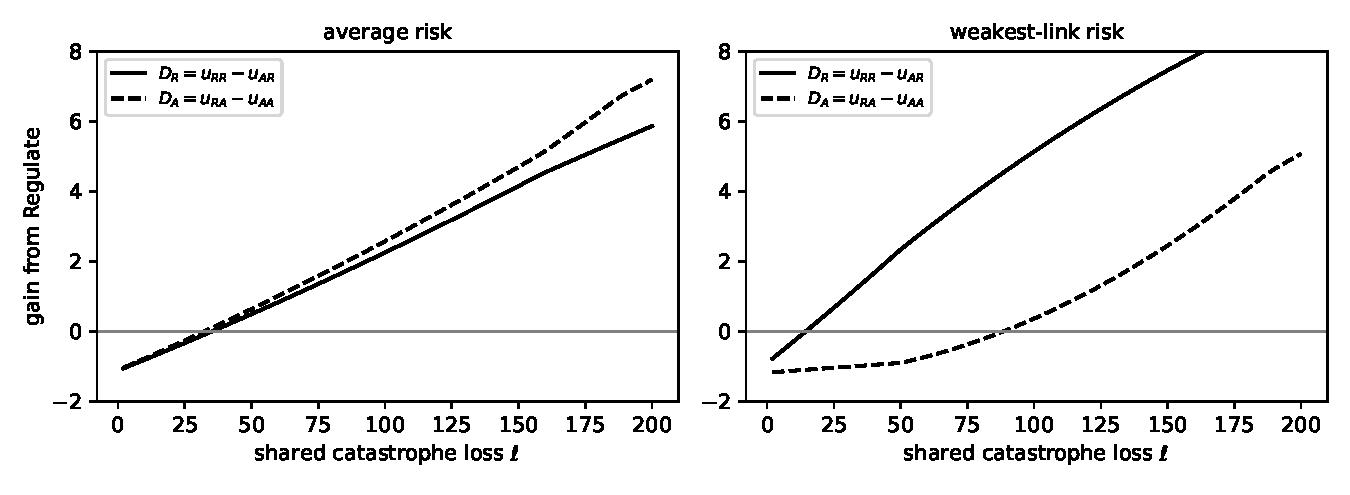
\includegraphics[width=\textwidth]{fig_taxonomy.pdf}
\caption{Gains from Regulate as functions of shared loss. Left: average risk~\eqref{eq:risk}, $D_A>D_R$ everywhere (PD, then Chicken, then dominant restraint). Right: weakest-link risk~\eqref{eq:wl}, $D_R>D_A$ (PD, then Stag Hunt, then dominant restraint).}
\label{fig:tax}
\end{figure}

\emph{Verification.} Table~\ref{tab:m} shows the thresholds as functions of $m$ under average risk. At $m=0.05$ restraint becomes dominant only above $\ell\approx168$; at $m=1$ above $\ell\approx35$. With $m=0.2$ and $\ell=30$, the regulated laboratory reaches only $s=0.02$ and the game is Deadlock; at $\ell=60$, where full monitoring makes restraint dominant, weak monitoring leaves a PD. The mild rise in $\ell^{\mathrm{mut}}$ between $m=0.8$ and $m=1$ is the endogenous-cost effect noted in Section~5.7.

\begin{table}[t]\centering\small
\caption{Thresholds as functions of monitoring precision (average risk, $\gamma=1$).}
\label{tab:m}
\begin{tabular}{l ccccccc}
\toprule
$m$ & 0.05 & 0.1 & 0.2 & 0.4 & 0.6 & 0.8 & 1.0\\
\midrule
$\ell^{\mathrm{uni}}(m)$ (PD below) & 167.9 & 128.7 & 72.4 & 38.8 & 32.9 & 31.7 & 32.2\\
$\ell^{\mathrm{mut}}(m)$ ($R$ dominant above) & 168.0 & 128.8 & 72.6 & 39.4 & 33.9 & 33.5 & 35.0\\
\bottomrule
\end{tabular}
\end{table}

\emph{Number of laboratories.} With $e=1$ and $\lambda=0.05$, symmetric equilibrium safety is $0.459$, $0.455$, $0.472$, $0.505$, $0.530$, $0.563$ for $n=2$, $3$, $4$, $6$, $8$, $12$: it falls from duopoly to triopoly and then rises, as~\eqref{eq:ncond} predicts. With $\lambda=1$ it falls monotonically ($0.880$ to $0.716$), and with $e=0$ and $\lambda=1$ it falls from $0.743$ to $0.164$. The \citet{armstrong2016} comparative static is a large-internalisation result.

\emph{Robustness.} The sign of $\Delt$ under average risk is a theorem; the width of the Chicken band is not. It is $(32.2,35.0)$ at $\rho=4$, $(42.0,60.6)$ at $\rho=8$, and $(44.6,59.7)$ at $\rho=16$: sanctions that create a larger speed asymmetry widen the band. A Tullock exponent $r$ above one (a more decisive race, $\pi_j=x_j^r/(x_j^r+x_k^r)$) widens it too---$(45.9,54.3)$ at $r=1.5$ and $(59.0,77.3)$ at $r=2$---while $r=0.5$ narrows it to $(17.1,17.6)$; $\Delt<0$ in every case. Decreasing returns to aggregate safety ($\gamma=0.5$ in the specification of the Section~5.4 remark) give $(19.7,44.1)$; increasing returns ($\gamma=2$) give a Stag Hunt band $(48.7,152.2)$. If the prize survives catastrophe, so that the laboratory earns $\pi_j\WL$ undiscounted, the thresholds move only to $(31.8,34.0)$. They are insensitive to the speed floor ($\varepsilon=0.01$: $(33.7,36.9)$; $\varepsilon=0.2$: $(27.5,29.4)$) and shift outward with the direct cost of regulation ($d=0$: $(26.5,28.9)$; $d=1$: $(54.2,58.9)$).

\emph{Behaviour.} With the falling-behind disutility of Section~5.5 and average risk, $\eta=2$ gives $\psi\approx-0.12$, $\Delt\approx+0.019$, and a Stag Hunt on $\ell\in(12.5,34.5)$; $\eta=5$ gives a Stag Hunt on $(11.0,89.7)$. The regulated laboratory, now behind, chooses safety of $0.19$--$0.25$ against a racing rival, below the $0.30$--$0.37$ it chooses against a regulated one. At $\eta=10$ the pressure to keep up drives every laboratory to the corner and the game is Deadlock throughout.

\subsection*{Where the camps stand}

The policy debate about racing divides, in the model's notation, on two parameters. One camp expects the first mover to gain a decisive and self-reinforcing advantage---automated AI research compounds the leader's lead, and the resulting economic and military edge persists \citep{bostrom2014,aschenbrenner2024,hendrycks2025}. In the model that is a high prize-to-loss ratio, $W/\ell$ of order one, usually paired with a low baseline catastrophe probability. The other camp expects the lead to be temporary---capabilities have diffused within months, and compute and energy are physical bottlenecks that do not self-improve---and takes loss of control seriously: $W/\ell$ of order $0.1$ or less, with $q_0$ of $0.2$ or more. Figure~\ref{fig:beliefs} maps the strategic form over $(W/\ell,\,q_0)$ for the three risk aggregation rules, holding $\ell=100$ and the other parameters at their illustrative values, so that a higher ratio also raises the laboratory stake $\WL=\sigma W$ and deepens the precipice.

\begin{figure}[t]\centering
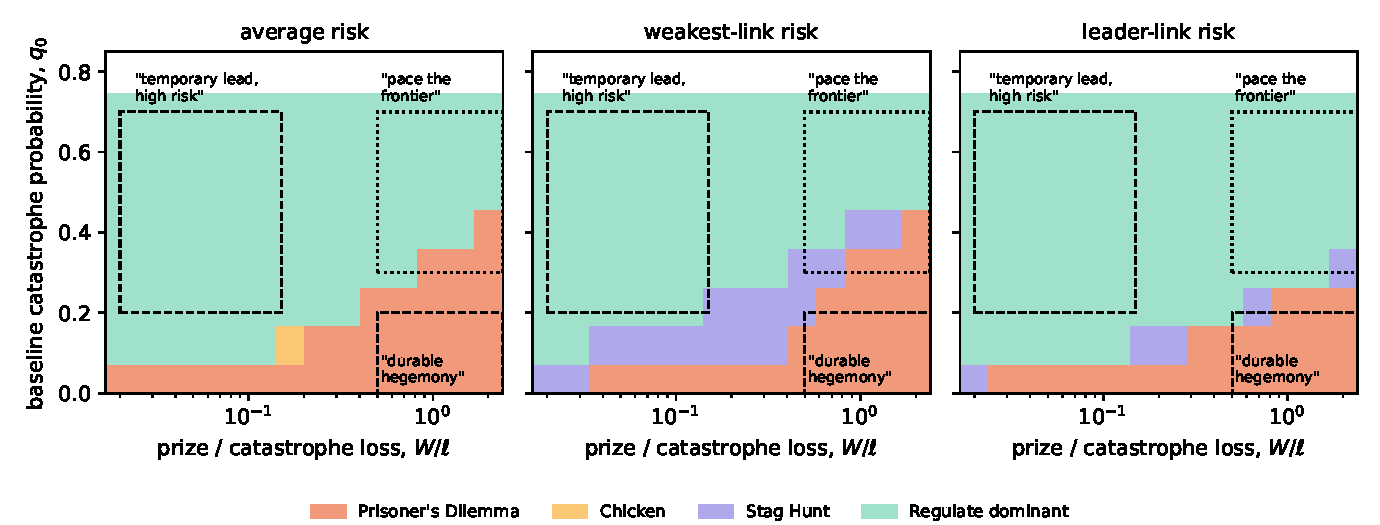
\includegraphics[width=\textwidth]{fig_beliefs.pdf}
\caption{Strategic form of the interstate game by beliefs about the prize-to-loss ratio and the baseline catastrophe probability, for three risk aggregation rules ($m=1$). Dashed boxes mark the regions occupied by the two camps of the policy debate; the dotted box marks the position of the pacing proposal \citep{amodei2026}.}
\label{fig:beliefs}
\end{figure}

Three features stand out. First, the boundary between racing and restraint is a ratio: restraint is an equilibrium roughly where $q_0$ exceeds a multiple of $W/\ell$. At $W/\ell=1$ that multiple is about $0.45$ under average risk, about $0.5$ under weakest-link risk, and about $0.35$ under leader-link risk---lower in the last case because a state's own laboratory's safety protects its own prize---so a state that believes the prize is as large as the catastrophe restrains only if it also believes catastrophe is roughly as likely as not. The durable-hegemony camp, which believes the first and not the second, sits in the Prisoner's Dilemma under every aggregation rule. Second, the temporary-lead, high-risk camp sits in dominant restraint under average and leader-link risk, but in or at the edge of the Stag Hunt band under weakest-link risk: for that camp the aggregation question decides whether the problem is trust or nothing at all. Third, the Chicken band under average risk is too thin to appear at this resolution, and the Stag Hunt band under leader-link risk is a diagonal sliver at the mild contest of the illustration but widens as the contest becomes decisive (Section~5.4), at which point the sanctioned laboratory's safety also collapses. A third position, that of the pacing proposal, holds both a large prize---its author endorses the view that a Chinese lead would be grave---and a serious catastrophe probability \citep{amodei2026}. That corner (dotted box) is dominant restraint under all three aggregation rules at the mild contest of the illustration, and moves into the Stag Hunt band under weakest-link risk at lower $q_0$ or under leader-link risk as the contest becomes decisive; the proposal's emphasis on verification and reciprocity is the Stag Hunt prescription, so its diagnosis and its remedy are consistent with each other and presuppose that a single unpaced laboratory keeps global risk high. The map does not adjudicate between the camps. It shows that their disagreement is about $W/\ell$ and $q_0$, that it maps onto different games rather than different readings of one game, and that the assurance framing is available only in a diagonal band whose location the technology sets.

\section{Discussion}

\subsection{What monitoring precision is}

The parameter $m$ stands for three things that the verification literature distinguishes. Inspectability is whether the regulated quantity---training compute, cluster ownership, evaluation results---can be observed at all \citep{shavit2023,sastry2024}. Detection is the probability $\delta$ that a violation, once inspectable, is caught \citep{wasil2024}. Leakage $\theta$ is the fraction of a jurisdiction's frontier activity that escapes its sanctions through third-country hosting, weight exfiltration, or open-weight release. Writing $e_i=(1-\theta)\,\delta\,m\,r_i$, all three enter the laboratory first-order condition only through $e_i$, so the bite and target thresholds of Proposition~2 scale by $1/[(1-\theta)\delta]$. Open-weight diffusion is the sharpest case: once weights are public, $\theta$ is close to one for that model and no domestic $(r,m)$ moves the relevant laboratory's incentives. Distillation of frontier models and theft of weights are leakage in a second sense: they erode a leader's capability lead, which Section~5.8 shows governs the leader's willingness to pace. Monitoring is also domestic before it is international. Embedded third-party evaluators with employee-level access raise $m$ within a jurisdiction and, where they may publish, raise $\lambda$ (Corollary~1); they do not by themselves raise the cross-border $m$ on which the interstate thresholds depend. A laboratory that adopts them unilaterally is choosing $m$ rather than receiving it, and the natural reading is a costly signal in the sense of \citet{kydd2000}: a laboratory that intends to comply bears the cost of being observed more cheaply than one that does not, so the choice can separate types and shift rivals' beliefs about compliance. A formal treatment would embed a signalling stage before the laboratory game; the baseline model, which fixes $m$, cannot represent this. Leakage does not impose a floor on residual risk in this specification; its effect is the scaling above. \citet{coe2020} explain why $m$ may stay low even when both states prefer it high: the inspection needed to detect skimping can reveal capability information that shifts beliefs about $W$ or relative position. The model treats that constraint as a bound on feasible $m$ rather than deriving it.

\subsection{What is and is not Putnam}

The model borrows the structure of Putnam's argument, in which international choices are constrained by domestic implementation, but not his mechanism. There are no ratifiers, no win-sets, and no domestic coalition politics; the domestic constraint is a single firm's best response to sanctions it may or may not face. Tsebelis's nested games, in which a player's apparently suboptimal move in one arena is optimal given a game in another, are the closer formal ancestor: a state that Regulates in a game where Regulate looks dominated may be responding to the laboratory game beneath it. The honest description is that the article formalises delegation across levels, not ratification.

\subsection{Nuclear analogies}

Shared extinction-scale loss creates mutual vulnerability. Three analogies travel with different fidelity. The laboratory stage is a peacetime arms race in the sense of \citet{glaser1997}: competitive investment under insecurity and prizes, with private agents and dual-use software as the disanalogies. The interstate stage is an arms-control problem in the sense of \citet{schelling1961}: management of incentives and information, where verification of training runs is the counterpart of counting warheads and is harder because compute is mobile and software is copyable. Crisis bargaining under mutual assured destruction is not modelled: it requires sequential moves, retaliatory technology, and private information \citep{powell1987}. Deterrence-by-sabotage postures \citep{hendrycks2025} would alter continuation values after acceleration and could move the game toward Chicken by a different route than the one derived here.

\subsection{Falsifiable implications}

The nesting claim predicts that announced restraint coexisting with unchanged training practices reflects effective regulation below the bite threshold---cheap $r$, low $m$, or high $\theta$---rather than a change in state preferences. It would be weakened by evidence that laboratory safety effort tracked interstate announcements under low measured monitoring capacity. The strategic-form result predicts that the character of interstate bargaining differs by risk aggregation rule: if unilateral restraint by one jurisdiction is observed to reduce perceived global risk substantially, the relevant game is Chicken-like and the observable politics should be about who moves first and burden-sharing; if unilateral restraint is perceived as nearly useless, the game is Stag Hunt-like and the politics should be about assurance. The competitor-count result predicts that the effect of entry on safety depends on the balance between diluted catastrophe internalisation and the declining marginal return to speed: entry reduces safety near a duopoly and wherever internalised losses are large, and can raise it at larger $n$ with weak liability; a local derivative in continuous $n$ and a discrete step from two to three laboratories can differ. Because frontier entry is gated by compute and talent, the testable form of this prediction concerns the step from two laboratories to three, not a large-$n$ limit; the entry that policy can affect is proximity to the frontier through distillation and diffusion, which enters the model as erosion and leakage rather than as an added competitor. The episode of pause rhetoric followed by continued scaling in 2023--2025 is consistent with the first prediction but is an illustration, not a test; establishing it would require institutional evidence on what regulators could observe. The sign of $\Delt$ can be estimated without a structural model, by conditional elicitation of catastrophe probabilities; Section~7.5 sets out that measurement and the two others the identification of the game requires. Estimating $\Delt$ tests a necessary condition for the ordering of incentives, not the game: establishing Chicken or a Stag Hunt also requires the payoff levels, enforcement costs, and winning prospects. The behavioural channel is testable directly, by applying designs like that of \citet{fernandez2026} to laboratory personnel, or observationally, from the response of safety staffing and evaluation timing to changes in a laboratory's relative position.

\subsection{What would have to be measured}

The model's practical content is a list of what must be known to tell which game is being played and how much enforcement, of what kind, it requires. Three quantities suffice; none is currently measured in the form the model needs. Two are beliefs to be elicited; the third is a requirement to be derived from them and then compared with what verification can feasibly deliver.

\begin{table}[!htb]
\centering\small
\caption{What determines the game, and how it could be measured}
\label{tab:measure}
\begin{tabular}{@{}>{\raggedright\arraybackslash}p{3.0cm}>{\raggedright\arraybackslash}p{3.5cm}>{\raggedright\arraybackslash}p{4.6cm}>{\raggedright\arraybackslash}p{3.5cm}@{}}
\toprule
Quantity & What it decides & How to establish it & What exists \\
\midrule
Prize-to-loss ratio $W/\ell$ and baseline probability $q_0$ & Where the thresholds fall; the bite and target thresholds; which camp a decision-maker is in (Figure~\ref{fig:beliefs}) & Only the ratio matters, so elicit ``how many times worse is catastrophe than a durable lead is good''; recover $W/\ell$ from officials' and laboratories' stated willingness to trade lead for risk; take $q_0$ from existing surveys & Rich on $q_0$ \citep{grace2024}; almost nothing on $W/\ell$, which is argued about in essays rather than measured \\
\addlinespace
Risk aggregation rule (sign of $\Delt$) & The \emph{type} of coordination problem: Chicken-side ($\Delt<0$) or Stag-Hunt-side ($\Delt>0$); whether unilateral restraint is useful or wasted; what kind of enforcement is needed & Elicit expert catastrophe probabilities conditional on both, neither, and exactly one leading jurisdiction enforcing frontier safety requirements; compute $\Delt=2Q_{AR}-Q_{RR}-Q_{AA}$; ask the one-restrains scenario both ways & Unconditional probabilities only \citep{grace2024}; no conditional elicitation \\
\addlinespace
Enforcement: required versus feasible ($e_0$, $m_{\mathrm{req}}$ against the ceiling on $m$, $\rho$, leakage $\theta$) & Whether the required enforcement can be had; Deadlock (Proposition~6) is the case in which the feasible ceiling lies below the bite threshold & Derive $e_0$ and $m_{\mathrm{req}}$ from the two quantities above; measure the ceiling directly: share of frontier training runs observable, detection probability, penalties available, share of frontier activity outside the jurisdiction & Compute-governance proposals \citep{sastry2024,shavit2023}; no published measurement of coverage \\
\bottomrule\end{tabular}
\end{table}

The order is one of logical dependence. The enforcement that is needed cannot be stated until beliefs and the rule are known: the bite threshold $e_0(\ell)$ and the required monitoring $m_{\mathrm{req}}$ are functions of $\ell$, $W$, $q_0$, and $\lambda$, and whether enforcement buys a Stag Hunt or a Chicken is a function of the aggregation rule. Beliefs and the rule therefore come first, and enforcement last---and enforcement is then partly a choice to be coordinated rather than a fact to be found. What remains a fact is the feasible ceiling on verification: what the technology, the mobility of compute, the copyability of weights, and the rival's willingness to be inspected allow. If that ceiling lies below the bite threshold the beliefs imply, no coordination delivers the agreement ($m_{\mathrm{req}}>1$ is exactly this case), and the instruments that must move are $\rho$, $\lambda$, or $W_L$, or the ceiling itself. The aggregation rule comes before the ratio because it changes the kind of problem rather than its location: on the Chicken side unilateral restraint reduces risk and the politics is about who moves first; on the Stag Hunt side it does not and the politics is about assurance. The ratio and the baseline probability locate the thresholds within whichever game obtains and are the substance of the present disagreement between the camps of Section~6. Reading the past runs the other way: to interpret announced restraint that changed nothing, one checks first whether enforcement lay below the bite threshold, because there Proposition~6 makes beliefs irrelevant to what happened. Two features of the elicitation matter. What the model needs is perceived risk---the beliefs on which states act---so the relevant respondents are the officials and laboratory decision-makers whose beliefs enter the game, with expert panels as a benchmark; and because a decisive-versus-accumulative distinction may hold across risk channels \citep{kasirzadeh2025}, the conditional questions should be asked separately for loss of control, misuse, and accumulated harm, since the rule may differ by channel and the interstate game is then a mixture.

\subsection{Limits}

Preferences $(W,\ell,q_0,\lambda,\Lam)$ are unobserved; the numerical section is illustrative only. The two-period extension is computed under regime commitment and, separately, under period-2 re-choice with a stated selection rule; neither is a full dynamic equilibrium analysis. Pure equilibria exist under weakest-link and leader-link risk (Lemma~4); existence in the behavioural extension, in the difference-form contest of Appendix~C, and for Tullock exponents other than one is verified numerically rather than proved, and a fine grid showing a single peak is evidence, not a proof of global concavity or uniqueness. The interstate stage is solved for one laboratory per state; with several laboratories per jurisdiction, $P_i$ is the sum of domestic contest probabilities and the identity in Lemma~3 continues to hold, but the sign of $\Delt$ must be recomputed. The baseline model is static and complete-information (the extensions in Appendices~C and~D relax the first in one respect each): private information about compliance and capability \citep{fearon1995,emery2024} and repeated play with reassurance \citep{kydd2005} are omitted, and both bear on whether the Chicken or Stag Hunt regions are resolved cooperatively. Monitoring precision is a parameter rather than a costly choice. Takeoff speed enters only through the risk aggregation rule and the decisiveness of the contest. A fast takeoff compresses the window in which $m$ can be raised, inflates effective $W$, and makes the race a first-passage problem with a finish line, in which the laboratory ahead at the threshold wins outright, rather than a Tullock contest in which speed shifts the odds continuously without ever securing the outcome; the strategies that matter in that setting---race to the front and pause at the threshold, or spend a lead on safety---require a dynamic model with at least two periods, which the static contest cannot represent. Deterrence or sabotage of a rival's programme \citep{hendrycks2025} is a third action absent from the $2\times2$. Firm--state relations differ across political economies; where the state can set $\rho$, $\lambda$, or $m$ directly, the feasible set is larger. The asymmetric case $m_U\neq m_C$ is computed in Appendix~E for the illustrative parameters only; the textbook names of Section~5 do not apply to asymmetric games, and the appendix classifies each state by its own best replies instead. Laboratories are symmetric in capability throughout. If one laboratory were persistently faster at every level of caution, the identity of Lemma~3 would fail state by state, because $Q_{AR}\neq Q_{RA}$ and the symmetric-profile win probabilities are no longer one half; but summed over the two states it survives as $\sum_i(D^i_R-D^i_A)=(W+2\Lam\ell)(Q_{AR}+Q_{RA}-Q_{RR}-Q_{AA})$, since within every profile the two states' prize terms add to $(1-Q)W$. The joint ordering of incentives is therefore still fixed by the risk aggregation rule; capability asymmetry decides only how that ordering is divided between the states. Computed cases are included in the replication code (\texttt{edge.py}) and are not reported.

\section{Who asks for regulation}

Frontier laboratories publicly warn of existential risk and call for regulation. Three hypotheses compete. Under the first, the laboratory internalises a large share of the catastrophe---through liability, reputation, mission, or the commercial value of a safety brand---so that in the model's terms its $\lambda$ is high. Under the second, the laboratory seeks rules that bind rivals more than itself, raising rivals' costs or removing competitors \citep{stigler1971,salop1983,yandle1983}. Under the third, it seeks to set the standard at its own current practice, converting a temporary technological advantage into an institutional one \citep{cset2025}. The model has no signalling equilibrium and cannot identify motives; what it can do is say which observations discriminate among the hypotheses, and predict how positions should sort by a laboratory's place in the race.

The documented record is consistent with all three. OpenAI has called for regulation in general while arguing against specific rules that would have bound it: in 2022--23 its chief executive urged global regulation while the company argued to European officials that its general-purpose models should not be classed as high risk, with several of its amendments reaching the final text \citep{perrigo2023}; it opposed California's SB~1047 in 2024 and sought federal pre-emption of state laws in 2025 \citep{fli2025,implicator2026}. Laboratories have favoured rules that act on rivals: a March 2025 OpenAI submission urged a ban on PRC-produced models in allied countries and stricter export controls \citep{wiggers2025}; the pacing proposal's protective measures---export controls, anti-distillation enforcement, weight security---act on rivals' speed \citep{amodei2026}. Where a laboratory has endorsed a rule that binds itself, the rule has been one it already satisfied or one scoped by size: Anthropic endorsed SB~53 as formalising existing practice, and the statute's strictest duties fall on developers with revenue above \$500 million \citep{anthropic2025sb53,brookings2026}; its embedded-evaluator commitment was made unilaterally with a call for governments to require rivals to match it \citep{amodei2026}. By 2026 both firms endorsed state bills as templates for a federal standard \citep{hill2026}.

Three observations from the model bear on the hypotheses. First, in every case computed, each laboratory's payoff is highest when only its rival is regulated, and both prefer mutual acceleration to mutual regulation unless $\lambda$ is large ($\lambda\ge0.5$ at $\ell=100$ in the symmetric baseline). Advocacy for rules that bind rivals---export controls, foreign-model bans, anti-distillation enforcement, size thresholds---is therefore consistent with any $\lambda$, and does not discriminate among the hypotheses. That these instruments are also, in Appendix~C, what makes a leader willing to pace is the coincidence \citet{yandle1983} called bootleggers and Baptists. Second, support for a rule that would cost the advocate something is consistent with a high $\lambda$ but not only with that: competitive advantage, reputation, and anticipated effects on rivals can explain it as well, and a rule the advocate already satisfies costs nothing and discriminates nothing. Establishing separation would require a signalling model with a specified type space, which the paper does not contain. Third, position in the race shapes which rules a laboratory wants. In the static lead game, mutual regulation lowers the leader's win probability and raises the follower's by the same amount, since the two sum to one; both laboratories lose payoff relative to mutual acceleration in the cases computed, and the leader loses more because it gives up more win probability. In the two-period game with erosion, by contrast, it is the follower \emph{state} that regulates in equilibrium, because a laboratory expecting to lose has the weakest return to speed and restraint is cheap for it. The prediction is that leaders demand lead-protecting instruments and followers demand universal pacing where their own cost of restraint is low---the substance of the critique that a slowdown ``buys time'' for a lagging firm \citep{eastern2026}, which the model accommodates without adopting.

Two implications follow for the analysis. If thresholds, tests, and approved auditors are shaped by incumbents, then sanction intensity $\rho$ is low for them and high for entrants, and regulation raises rivals' costs by construction---a channel distinct from the verification wedge, requiring not that $m$ be low but that it be asymmetric \citep{salop1983}. And evaluators chosen and paid by a laboratory shift states' beliefs about $q_0$ (Figure~\ref{fig:beliefs}) in the direction the laboratory's position favours, so their credibility rests on independence rather than access. None of this implies that the risk claims are false; it implies that the truth of a risk claim cannot be assessed from the fact that a laboratory makes it, and that the design question for a regulator is whether the rules being asked for would bind the asker.

\section{Policy implications}

The results support the following conclusions, each conditional on the mechanism that generates it and on the parameter ranges analysed. They are conditional in a second sense as well: which instrument is appropriate depends on which game obtains and on how much enforcement it requires, and Section~7.5 shows how to establish both---beliefs about the prize-to-loss ratio and the baseline probability, and the risk aggregation rule, first; the enforcement they require, set against what verification can feasibly deliver, last. The recommendations below should be read as a map from that diagnosis to an instrument, not as a list to be applied in full.

\emph{Enforcement before verification.} At the laboratory margin, liability and expected sanctions are substitutes; monitoring makes sanctions effective. A given safety target can be reached with less monitoring if liability is higher, and the target may be unreachable by monitoring alone. Liability is therefore not a weaker instrument than monitoring; it is a substitute for it at the laboratory margin. What the model does identify as empty is a Regulate announcement with $m$ below the bite threshold, which has no effect on laboratory incentives at all. Civil liability and mandatory insurance for frontier-scale harms, windfall or profit-sharing commitments that lower the private value of unconstrained racing \citep{okeefe2020,askell2019}, and evaluation gates whose failure is costly in licence or compute terms all raise $\lambda$ or $\rho$.

\emph{Verification without sanction is a signal, not an instrument.} Embedded evaluators raise $m$ and, through publication, $\lambda$; until a regulator attaches consequences to what they find, $e=mr$ is unchanged (Corollary~1). The first step of the pacing proposal \citep{amodei2026} is therefore an investment in the verifiability of later steps and a costly signal to rivals, and its effect on safety at the laboratory margin runs through reputation until regulation follows. That is consistent with the proposal's own claim that regulation is the effective route.

\emph{A lead is spent unless the rival is also constrained, and the constraint must be binding.} In the examples of Appendix~C, a leader's unilateral slowdown shrinks its lead and is self-limiting, while committed mutual regulation widens the lead and makes deep pacing consistent with winning; a regime that will be re-chosen once the lead is observed invites the follower to race first and unravels. Protecting the lead through export controls, anti-distillation enforcement, and weight security matters because erosion decides whether the leader is willing to pace at all. If a speed limit on self-improvement reduces the decisiveness of the race---an additional modelling assumption---it is the one instrument in the model that narrows the assurance band and keeps the regulated laboratory's safety from collapsing.

\emph{Verification selects the game.} Compute reporting, chip and cluster know-your-customer requirements, third-party audit of training runs, and hardware-backed monitoring raise $m$ \citep{shavit2023,sastry2024,baker2023}. Their effect in the model is not to add a lever alongside the others but to move the thresholds at which restraint becomes an equilibrium and then dominant. At low $m$ no level of perceived risk makes restraint rational. The monitoring literature's transparency--security tradeoff bounds how far this can be pushed.

\emph{Verification of the rival.} Appendix~E adds a computed reason why cross-border verification comes before any agreement. Where one state's enforcement is below its bite threshold, its promise of restraint is empty whatever it announces, and the well-enforced state is left either to restrain alone (average risk) or to race (weakest-link risk). A state confident in its own enforcement therefore gains from raising the rival's, which is what makes verification of the rival the enforced state's demand rather than a concession.

\emph{Which coordination problem.} Under average risk, the coordination problem that emerges once perceived risk is high enough is Chicken. Its instruments are commitment devices and burden-sharing: simultaneous, verified, reciprocal moves that avoid the asymmetric equilibria in which one state bears the cost of restraint \citep{schelling1960}, and institutions that make first-mover commitment to acceleration costly. Chicken also implies that unilateral restraint is individually rational above $\ell^{\mathrm{uni}}$, so a state confident that risk is high should regulate even without reciprocity. Under weakest-link risk, or where laboratories cut safety when they fall behind, the problem is a Stag Hunt: unilateral restraint is nearly useless, and the instruments are reassurance and costly signals that shift beliefs about rival compliance \citep{kydd2000}. Assurance-based proposals are therefore conditional on an empirical premise---about the risk aggregation rule or about laboratory behaviour---that has not been established; so is the claim that unilateral restraint is futile. Coalition-first clubs among allied jurisdictions \citep{schelling1961} are consistent with either case, but for different reasons: they lower the burden-sharing problem in Chicken and raise expected compliance in the Stag Hunt.

\emph{Antitrust and legality.} Industry-wide evaluation gates or reciprocal compute caps among competing laboratories can raise antitrust exposure; statutory licensing faces administrative and trade-law frictions. These constrain feasible $(\rho,m)$ and the calendar time available to raise them, and they weigh more heavily where laboratories are private and $\lambda$ is low.

\section{Conclusion}

The persistent question in AGI strategy debates---is the race a Prisoner's Dilemma or a trust dilemma?---is not well posed at the level at which it is usually asked. States do not race; their laboratories do, under incentives the state only partly controls and can only partly observe. Writing the interstate game as the reduced form of the laboratory game yields three results. Laboratories under-provide safety below an explicit internalisation threshold, and regulation reaches them only above an explicit monitoring threshold that need not lie in the feasible range. The strategic form of the interstate game is fixed by a single derived quantity, the risk convexity $\Delt$. Under average risk it is never an assurance game: the discouragement of a regulated laboratory facing a racing rival makes unilateral restraint less risky than single-layer assurance models assume, and the coordination problem that emerges at high perceived risk in the illustration is Chicken. Under weakest-link or leader-link risk, or when laboratories cut safety as they fall behind, the examples computed produce a Stag Hunt. The PD-versus-trust-dilemma debate is therefore a disagreement about the shape of catastrophe risk and the behaviour of frontier laboratories, and it should be argued on those grounds. And monitoring precision moves the thresholds between regions roughly fivefold in the illustration, so that verification shifts which game states play before any question of equilibrium selection arises.

The methodological moral is discipline about levels. Before asserting that the AGI race has a given strategic form, specify the laboratory game, solve it under every regulatory profile, and let the interstate payoffs follow. Different answers at different levels are not inconsistency; they are what nesting predicts. The same discipline says what to establish, and in what order: how large the prize is believed to be relative to the loss and how likely catastrophe is thought to be; how one laboratory's carelessness adds to everyone's risk; and only then how much enforcement those beliefs require, set against how much verification can deliver---because the requirement cannot be stated without the beliefs, and the game cannot be named without the rule. For conflict research the case is a hard test of arms-control theory under private agents, dual-use software, and contested monitoring. The model's answer is that the first-order questions are empirical---how convex is catastrophe risk in the breadth of compliance, how do frontier laboratories respond to falling behind, and what can regulators observe---and that the familiar strategic labels should be conclusions from those questions, not premises.

\appendix
\section{Proofs}

\subsection{Lemma 1 (regularity)}
Fix $s_k$ and $e_j$. With $\gamma=1$, $1-Q=1-q_0+\tfrac{q_0\alpha}{2}(s_j+s_k)$ is affine and increasing in $s_j$; $\pi_j=x_j/(x_j+x_k)$ satisfies $\partial\pi_j/\partial s_j=-x_k/X^2<0$ and $\partial^2\pi_j/\partial s_j^2=-2x_k/X^3<0$. For a product $h=ab$ with $a>0$ affine increasing and $b$ decreasing concave, $h''=ab''+2a'b'<0$. Hence $(1-Q)\pi_j\WL$ is strictly concave in $s_j$; the remaining terms of~\eqref{eq:lab} are concave or linear, so $u_j$ is strictly concave. Best responses are therefore single-valued and continuous on the compact convex set $[0,1]$ (the floor $\varepsilon$ keeps $\pi_j$ continuous at $s_j=s_k=1$), and Brouwer's theorem gives a pure equilibrium. At a symmetric profile with $e_U=e_C$, an equilibrium is a zero of $F(\cdot;e,2)$ in~\eqref{eq:symfoc} or the corner $0$ (if $F(0)\le0$) or $1$ (if $F(1)\ge0$); since $F$ is strictly decreasing in $s$---each of $(1-Q(s))/(1-s+\varepsilon)$ and $\kappa s$ is increasing---the symmetric equilibrium is unique.

\subsection{Proposition 1 (precipice)}
The symmetric equilibrium is a zero of $F(\cdot;e,n)$ or a corner. Since $F$ is strictly decreasing in $s$, the three cases are exhaustive and exclusive: the corner $s=0$ iff $F(0;e,n)\le0$, the corner $s=1$ iff $F(1;e,n)\ge0$, and otherwise a unique interior root. Substituting $Q(0)=q_0$ gives
\[
\WL\Bigl[\frac{q_0\alpha}{n^2}-\frac{(1-q_0)(n-1)}{n^2(1+\varepsilon)}\Bigr]+\frac{\lambda q_0\alpha\ell}{n}+\rho e\le0,
\]
which rearranges to~\eqref{eq:lambdabar}. On the interior, since $F$ is decreasing in $s$ and weakly increasing in $e,\lambda,\rho,\ell$ (strictly when the relevant coefficient is positive), the implicit function theorem gives the stated monotonicity; at the corners the equilibrium is locally constant, which gives the weak statements; and $\partial F/\partial\WL$ is the bracket in~\eqref{eq:symfoc}.

\subsection{Proposition 2 (implementation thresholds)}
With a common $s$ and $n=2$, $Q(s)=q_0(1-\alpha s)$ so $dQ/ds=-q_0\alpha$, and the first-order condition of~\eqref{eq:sc} is $q_0\alpha W/2+\Lam q_0\alpha\ell-\kappa s=0$, giving $s^c$. Under $r=(1,1)$, $e=m$ and the symmetric equilibrium solves $F(s;m,2)=0$ with $F$ increasing in $m$ at rate $\rho$ and decreasing in $s$. Thus $s^*(m)=0$ iff $F(0;m,2)=B+\rho m\le0$; if $B<0$ this is $m\le-B/\rho$, and if $B\ge0$ it holds only at $m=0$ when $B=0$ and never when $B>0$. Likewise $s^*(m)\ge s^c$ iff $F(s^c;m,2)\ge0$ iff $m\ge-F(s^c;0,2)/\rho$, so the target is attained iff $m\ge m_{\mathrm{req}}=\max\{0,-F(s^c;0,2)/\rho\}$. Expanding $F(s^c;0,2)$ gives~\eqref{eq:ebar}. Where $m_{\mathrm{req}}>0$, since $F(s;0,2)$ is decreasing in $s$ it is increasing in $s^c$; the remaining comparative statics are read from~\eqref{eq:ebar} directly, and all vanish where the threshold is capped at zero or the target at one.

\subsection{Proposition 3 (competitor count)}
Differentiating~\eqref{eq:symfoc} in $n$ at fixed $s$, using $\tfrac{d}{dn}\tfrac{n-1}{n^2}=\tfrac{2-n}{n^3}$,
\[
\frac{\partial F}{\partial n}=\WL\left[\frac{(1-Q)(n-2)}{(1-s+\varepsilon)n^3}-\frac{2q_0\alpha}{n^3}\right]-\frac{\lambda q_0\alpha\ell}{n^2}.
\]
Since $\partial F/\partial s<0$, $\operatorname{sign}(ds^*/dn)=\operatorname{sign}(\partial F/\partial n)$, and multiplying by $n^3$ gives~\eqref{eq:ncond}. At $n=2$ the bracket equals $-2q_0\alpha<0$.

\subsection{Lemma 2 (cross effects)}
From~\eqref{eq:foc}, with $\partial\pi_j/\partial s_k=x_j/X^2$, $\partial(1-Q)/\partial s_k=q_0\alpha/2$, and $\partial^2\pi_j/\partial s_j\partial s_k=(x_j-x_k)/X^3$,
\[
\frac{\partial^2u_j}{\partial s_j\partial s_k}=\frac{q_0\alpha}{2}\WL\frac{x_j}{X^2}-\frac{q_0\alpha}{2}\WL\frac{x_k}{X^2}+(1-Q)\WL\frac{x_j-x_k}{X^3},
\]
which is~\eqref{eq:cross}. For general $\gamma$ the additional term is $-\partial^2Q/\partial s_j\partial s_k\,(\pi_j\WL+\lambda\ell)$ with $\partial^2Q/\partial s_j\partial s_k=-\tfrac{q_0\alpha\gamma(\gamma-1)}{4}\Sh^{\gamma-2}$.

\subsection{Proposition 4 (strategic form)}
The four cases are the standard ordinal classification of a symmetric $2\times2$ game by the signs of $D_R$ and $D_A$ \citep{snyder1971}; the necessity of $\Delt>0$ for case (iii) and $\Delt<0$ for case (iv) follows from Lemma~3, and $u_{RR}>u_{AA}$ iff $d<(Q_{AA}-Q_{RR})(W/2+\Lam\ell)$ by direct subtraction.

\subsection{Lemma 3 (identity)}
Subtracting,
\begin{align*}
D_R-D_A&=\Bigl[(1-Q_{RR})\tfrac W2-\Lam Q_{RR}\ell-d\Bigr]-\Bigl[(1-Q_{AR})\pi^{AR}_AW-\Lam Q_{AR}\ell\Bigr]\\
&\quad-\Bigl[(1-Q_{AR})(1-\pi^{AR}_A)W-\Lam Q_{AR}\ell-d\Bigr]+\Bigl[(1-Q_{AA})\tfrac W2-\Lam Q_{AA}\ell\Bigr]\\
&=\tfrac W2\bigl[2-Q_{RR}-Q_{AA}\bigr]-(1-Q_{AR})W+\Lam\ell\bigl[2Q_{AR}-Q_{RR}-Q_{AA}\bigr]
=\Bigl(\tfrac W2+\Lam\ell\Bigr)\Delt.
\end{align*}
Under leader-link accounting the prize terms are $\tfrac12(1-q(s_{RR}))W$, $\tfrac12(1-q(s_{AA}))W$, $\pi^{AR}_A(1-q(s^{AR}_A))W$ and $(1-\pi^{AR}_A)(1-q(s^{AR}_R))W$. Since $\pi_A(1-q_A)+\pi_R(1-q_R)=1-Q^{\mathrm{LL}}_{AR}$ and $\tfrac12(1-q(s_{RR}))+\tfrac12(1-q(s_{AA}))=1-\tfrac12(Q_{RR}+Q_{AA})$, the same computation gives the same identity.

\subsection{Proposition 5 (no assurance game under average risk)}
Let $f(s_k)$ denote the best response of an unregulated laboratory ($e_j=0$) to rival safety $s_k$, and $g(s_k)$ that of a regulated laboratory ($e_j=m$). By Lemma~1 both are single-valued and continuous on $[0,1]$, corners included. Three facts are used.

(a) \emph{Order.} $g\ge f$ pointwise: the sanction adds $\rho m>0$ to the marginal return~\eqref{eq:foc} at every $s_j$, so the maximiser of a strictly concave objective weakly rises.

(b) \emph{Single crossing.} $f(s)=s$ iff $s$ is a symmetric equilibrium of the subgame with $e=0$, which is unique by Lemma~1; call it $s_{AA}$. Moreover $f(s)\ge s$ on $[0,s_{AA}]$ and $f(s)\le s$ on $[s_{AA},1]$. If $f(s')<s'$ for some $s'<s_{AA}$, let $s_1=\sup\{s\le s':f(s)\ge s\}$, which exists because $f(0)\ge0$; by continuity $f(s_1)=s_1$, a second fixed point, a contradiction. The claim on $[s_{AA},1]$ follows symmetrically from $f(1)\le1$. The same statements hold for $g$ with fixed point $s_{RR}$.

(c) \emph{Slope.} Where the best response is interior, its derivative in $s_k$ has the sign of the cross partial~\eqref{eq:cross}, which by Lemma~2 is the sign of $s_k-s_j$; where it is at a corner it is locally constant. Hence $f$ is nonincreasing on $[0,s_{AA}]$, where $f(s)\ge s$, and nondecreasing on $[s_{AA},1]$, where $f(s)\le s$; likewise $g$ is nonincreasing on $[0,s_{RR}]$ and nondecreasing on $[s_{RR},1]$.

From (a) and (b), $g(s_{AA})\ge f(s_{AA})=s_{AA}$, so $s_{RR}\ge s_{AA}$.

An equilibrium of the asymmetric subgame is a pair with $s_R=g(s_A)$ and $s_A=f(s_R)$, i.e.\ a fixed point of $\varphi:=f\circ g$. \emph{Existence:} $\varphi(s_{AA})=f(g(s_{AA}))\ge f(s_{AA})=s_{AA}$, because $g(s_{AA})\ge s_{AA}$ and $f$ is nondecreasing on $[s_{AA},1]$; and $\varphi(s_{RR})=f(s_{RR})\le s_{RR}$ because $s_{RR}\ge s_{AA}$. By continuity $\varphi$ has a fixed point in $[s_{AA},s_{RR}]$. \emph{Location:} for $s_A<s_{AA}$, $g(s_A)\ge g(s_{AA})\ge s_{AA}$ since $g$ is nonincreasing on $[0,s_{RR}]\supseteq[0,s_{AA}]$, so $\varphi(s_A)\ge f(s_{AA})=s_{AA}>s_A$; for $s_A>s_{RR}$, $g(s_A)\le s_A$ and $g(s_A)\ge g(s_{RR})=s_{RR}\ge s_{AA}$ since $g$ is nondecreasing on $[s_{RR},1]$, so $\varphi(s_A)=f(g(s_A))\le g(s_A)\le s_A$ with equality only if $g(s_A)=s_A$, i.e.\ $s_A=s_{RR}$, excluded. Hence every asymmetric equilibrium has $s^{AR}_A\in[s_{AA},s_{RR}]$, and then $s^{AR}_R=g(s^{AR}_A)\ge g(s_{RR})=s_{RR}$ because $g$ is nonincreasing on $[0,s_{RR}]$. This is the ordering in the proposition. Both differences in~\eqref{eq:psi} are nonnegative, so $\psi\ge0$, $\Delt=-q_0\alpha\psi\le0$, and $D_R\le D_A$ by Lemma~3; a Stag Hunt requires $D_R>0>D_A$, which is impossible.

\subsection{Remark on increasing returns to aggregate safety}
Adding and subtracting $2g(\tilde s)$ gives the decomposition. For $\gamma\ge1$, $g''(x)=-q_0\alpha\gamma(\gamma-1)x^{\gamma-2}\le0$, so $g$ is concave and Jensen's inequality gives $g(\tilde s)\ge\tfrac12[g(s_{RR})+g(s_{AA})]$, with equality when $\gamma=1$; the inequality reverses for $\gamma\le1$. Since $g$ is decreasing and $\Sh_{AR}-\tilde s=\psi/2$, the second term has the sign of $-\psi$. The complementarity term follows from the last line of the proof of Lemma~2; it is one term of the total cross partial, whose sign is not established in general.

\subsection{Corollary 3 (pedagogical limit) and risk dominance}
With $u_{RR}=W/2$, $u_{AA}=(1-q)W/2-q\ell$, $u_{AR}=(1-q)W-q\ell$, $u_{RA}=-q\ell$: $D_R=q(W+\ell)-W/2\ge0$ iff $q\ge W/[2(W+\ell)]$; $D_A=-(1-q)W/2<0$ for all $q<1$. Risk dominance of $(A,A)$ requires $-D_A\ge D_R$, i.e.\ $(1-q)W/2\ge q(W+\ell)-W/2$, i.e.\ $q\le 2W/(3W+2\ell)$, and $2W/(3W+2\ell)-W/[2(W+\ell)]=W(W+2\ell)/[2(3W+2\ell)(W+\ell)]>0$. The mixed equilibrium has each state regulating with probability $p^*=-D_A/(D_R-D_A)$.

\subsection{Lemma 4 (existence for the nonlinear aggregation rules)}
\emph{Statement.} Let $r=1$. (a) Under weakest-link risk~\eqref{eq:wl}, $u_j$ is strictly concave in $s_j$ for every $s_k$ and $e_j$, so a pure-strategy equilibrium exists in every regulatory profile. (b) Under leader-link risk~\eqref{eq:ll}, $u_j$ is strictly concave in $s_j$ for every $s_k$ and $e_j$, so a pure-strategy equilibrium exists in every regulatory profile.

\emph{Proof.} A product $h=ab$ of nonnegative functions with $a$ increasing and concave and $b$ decreasing and concave is concave, since $h''=a''b+2a'b'+ab''$ and each term is nonpositive. (a) The soft minimum $S_\tau(s)=-\tau\log\tfrac12(e^{-s_U/\tau}+e^{-s_C/\tau})$ is increasing in each argument and concave, being the negative of a log-sum-exp composed with a linear map; hence $1-Q^{\mathrm W}=1-q_0+q_0\alpha S_\tau$ is positive, increasing, and concave in $s_j$, and $Q^{\mathrm W}$ is convex. With $\pi_j$ positive, decreasing, and concave in $s_j$ ($\partial^2\pi_j/\partial s_j^2=-2x_k/X^3<0$), the prize term $(1-Q^{\mathrm W})\pi_j\WL$ is concave, $-\lambda Q^{\mathrm W}\ell$ is concave, and the remaining terms are strictly concave or linear. Best responses are therefore single-valued and continuous on $[0,1]$, and Brouwer's theorem gives a pure equilibrium. (b) The prize term $\pi_j(1-q_j)\WL$ is the product of $\pi_j$ with the positive increasing linear function $1-q_0+q_0\alpha s_j$, hence concave. For the risk term, write $x_j=1-s_j+\varepsilon$, so that $q_j=a+bx_j$ with $b=q_0\alpha$ and $a=q_0(1-\alpha-\alpha\varepsilon)$, and $Q^{\mathrm{LL}}=(x_jq_j+x_kq_k)/(x_j+x_k)$. Differentiating in $x_j$ and using $x_kq_k=ax_k+bx_k^2$ gives $\partial Q^{\mathrm{LL}}/\partial x_j=b-2bx_k^2/(x_j+x_k)^2$ and hence
\[
\frac{\partial^2Q^{\mathrm{LL}}}{\partial s_j^2}=\frac{\partial^2Q^{\mathrm{LL}}}{\partial x_j^2}=\frac{4q_0\alpha\,x_k^2}{(x_j+x_k)^3}>0
\]
for every $(s_j,s_k)$. So $Q^{\mathrm{LL}}$ is strictly convex in own safety everywhere, $-\lambda Q^{\mathrm{LL}}\ell$ is concave, and with the quadratic cost $u_j$ is strictly concave. Best responses are single-valued and continuous, and Brouwer's theorem gives a pure equilibrium in every profile.

\subsection{Proposition 6 (regulation below the bite threshold)}
If $B<0$ and $m\le-B/\rho$ then $F(0;m,2)\le0$, so in every profile the profile $(0,0)$ satisfies both laboratories' corner conditions; by the ordering of Proposition~5 it is the unique equilibrium of each profile. Then $Q$ and $\pi_i=\tfrac12$ are the same in all four cells, and the only differences are the direct costs: $u_{RR}=u_{AA}-d$, $u_{RA}=u_{AA}-d$, $u_{AR}=u_{AA}$, so $D_R=D_A=-d$ and $u_{RR}<u_{AA}$.

\section{Numerical procedure}

Laboratory equilibria are computed for each of the four regulatory profiles by iterated best response with damping, where each best response is the unique zero of the exact marginal condition~\eqref{eq:foc} (or the corner where the marginal condition has no interior zero), solved by bracketing to tolerance $10^{-13}$; the fixed point is accepted at $10^{-12}$. Continuation values are then evaluated from~\eqref{eq:state}, and $D_R$, $D_A$, $\Delt$, and $\psi$ are computed from them. The identity in Lemma~3 was verified to machine precision at every point as a check on the solver. Thresholds $\ell^{\mathrm{uni}}$, $\ell^{\mathrm{mut}}$, and $\ell_{rd}$ are roots of $D_A$, $D_R$, and $D_R+D_A$ in $\ell$. For weakest-link and leader-link risk, the increasing-returns remark, Tullock exponents $r\neq1$, and the behavioural extension, best responses are computed by grid search on 401 points followed by local refinement; the number of local maxima of the objective on the grid is recorded and was one in every reported equilibrium, which is numerical evidence of single-peakedness, not a proof of concavity or uniqueness. All four regulatory profiles are solved jointly, including asymmetric laboratory choices. Each printed payoff, $D_A$, $D_R$, $\Delt$, and classification is computed from the same stored equilibrium, and the identity of Lemma~3 is verified at every point. Grids are refined around game transitions when thresholds are reported. The random search draws 400 parameter vectors uniformly from $\sigma\in[0.2,1]$, $\kappa\in[1,15]$, $q_0\in[0.02,0.6]$, $\alpha\in[0.3,1]$, $\varepsilon\in[0.01,0.3]$, $\lambda\in[0,0.3]$, $\rho\in[0.5,10]$, $m\in[0.1,1]$, $\ell\in[1,300]$, $d\in[0,1]$, $\Lam\in[0.2,1]$, with $W=10$ and $\gamma=1$. The code is supplied as supplementary material.


\section{Extension: the lead as a stock}

The pacing proposal \citep{amodei2026} rests on a claim the static model cannot evaluate: that a laboratory ahead of its rivals can slow down by up to the size of its lead without losing the race, and that protecting the lead is what creates room to pace \citep{amodei2026}. This appendix specifies a two-period model in which that claim can be assessed and reports numerical results.

\emph{Primitives.} The lottery contest~\eqref{eq:contest} cannot represent a lead, since any slowdown lowers the win probability. Replace it with the difference-form contest of \citet{hirshleifer1989},
\begin{equation}
\pi_U=\mathcal L\!\left(\frac{x_U-x_C+\delta}{\varsigma}\right),\qquad \mathcal L(z)=\frac{1}{1+e^{-z}},
\label{eq:diff}
\end{equation}
where $\delta$ is the leading laboratory's capability lead and $\varsigma$ indexes noise; as $\varsigma\to0$ a lead larger than the slowdown keeps $\pi_U$ at one. The cross-effect lemma for the Tullock contest does not apply to~\eqref{eq:diff}; all results below are computed. Risk is leader-link with the winner-causes-catastrophe accounting of~\eqref{eq:ll}. There are two periods and no discounting. In period~1 laboratories choose $s^1_j$; there is no prize, period-1 risk is $Q^1=Q^{\mathrm{LL}}(s^1;\delta_0)$ evaluated at the current lead, and catastrophe is absorbing. The lead carried into period~2 is
\begin{equation}
\delta_1=\delta_0+\tau\,(x^1_U-x^1_C)-\theta,
\label{eq:leadlaw}
\end{equation}
where $\tau$ converts speed differences into lead and $\theta\ge0$ is erosion from distillation and weight theft. Period~2 is the static game at $\delta_1$: laboratories choose $s^2_j$, the race resolves, and prizes and losses realise as in~\eqref{eq:ll}. States commit to a regime $r=(r_U,r_C)$ for both periods and bear $d\,r_i$ in each. Lifetime objectives are
\[
U_j=-\tfrac{\kappa}{2}(s^1_j)^2-\lambda Q^1\ell-\rho e_j(1-s^1_j)+(1-Q^1)\,u^2_j(\delta_1),\qquad
V_i=-\Lam Q^1\ell-d\,r_i+(1-Q^1)\,V^2_i(\delta_1),
\]
where $u^2_j$ and $V^2_i$ are period-2 equilibrium payoffs. Period-2 laboratory equilibria are computed by damped iterated best response on a 201-point grid from a symmetric start, on a grid of leads $\delta_1\in[-0.8,1.6]$ (step $0.1$), and interpolated linearly; they were unique in every case examined. Period-1 equilibria are computed the same way with the interpolated continuation; where the period-1 game has several equilibria, selection is by inertia---iteration starts from the equilibrium at the previous value of $\delta_0$---which removes most, not all, of the discontinuities in $\delta_0$. The interstate stage is a $2\times2$ game in regimes; all four regimes are solved and pure equilibria reported.

\emph{Results.} Figure~\ref{fig:lead} and Table~\ref{tab:lead} report a decisive race ($\varsigma=0.1$, $\ell=60$, other parameters as in Section~6); the findings also hold at $\varsigma=0.3$ and $\ell=100$.

\begin{figure}[t]\centering
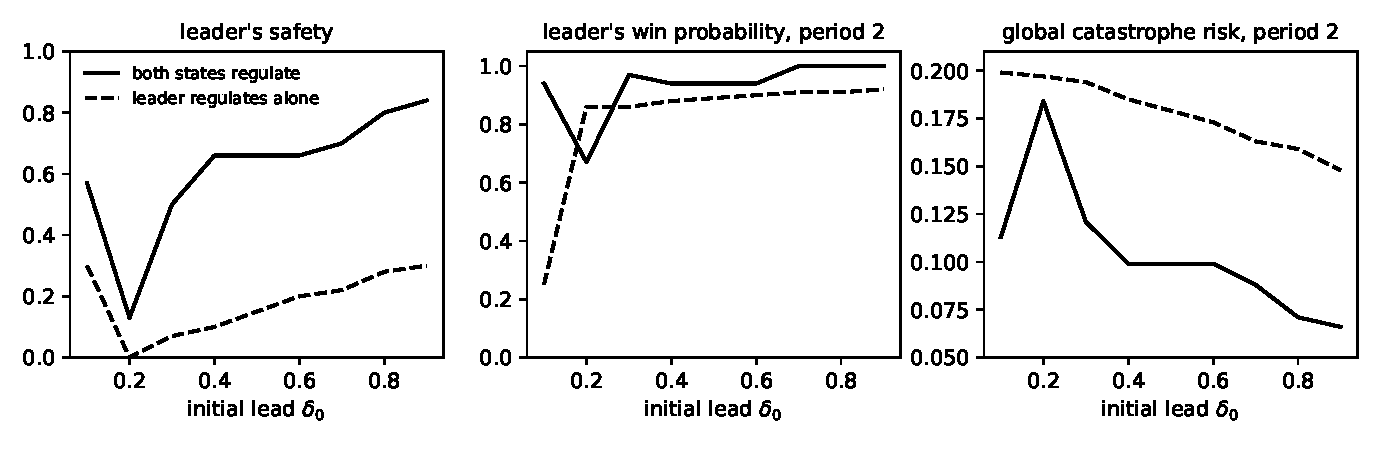
\includegraphics[width=\textwidth]{fig_lead.pdf}
\caption{Pacing within the lead, no erosion ($\theta=0$, $\varsigma=0.1$, $\ell=60$). When the leader regulates alone it paces little and the lead shrinks; when both states regulate the lead widens, the leader paces deeply while keeping a win probability above $0.93$, and global risk roughly halves.}
\label{fig:lead}
\end{figure}

\begin{table}[t]\centering\footnotesize\setlength{\tabcolsep}{3.5pt}
\caption{Two-period lead-as-stock model, leader-link risk. $s^1$ is period-1 safety, $\delta_1$ the lead carried forward, $s^2_U$ and $\pi^2_U$ the leader's period-2 safety and win probability, $Q^2$ period-2 risk. ``none'': no pure-strategy equilibrium in regimes. $\ast$: the leader loses the lead and capitulates.}
\label{tab:lead}
\begin{tabular}{cccc c ccc c cccc}
\toprule
& & & & & \multicolumn{3}{c}{leader regulates alone} & & \multicolumn{4}{c}{both regulate}\\
\cmidrule{6-8}\cmidrule{10-13}
$\varsigma$ & $\ell$ & $\theta$ & $\delta_0$ & equilibrium & $s^1_U$ & $\pi^2_U$ & $Q^2$ & & $s^1$ & $\delta_1$ & $s^2_U$, $\pi^2_U$ & $Q^2$\\
\midrule
0.1 & 60 & 0 & 0.3 & $(R,R)$ & 0.07 & 0.86 & 0.194 & & (0.19, 0.41) & 0.53 & 0.50, 0.97 & 0.121\\
0.1 & 60 & 0 & 0.6 & $(R,R)$ & 0.20 & 0.90 & 0.173 & & (0.49, 0.54) & 0.65 & 0.66, 0.94 & 0.099\\
0.1 & 60 & 0 & 0.9 & $(R,R)$ & 0.30 & 0.92 & 0.148 & & (0.74, 0.80) & 0.96 & 0.84, 1.00 & 0.066\\
0.1 & 60 & 0.2 & 0.3 & none & 0.59 & 0.00 & 0.166 & & (0.26, 0.71) & 0.55 & 0.57, 0.94 & 0.113\\
0.1 & 60 & 0.2 & 0.6 & $(R,R)$ & 0.10 & 0.88 & 0.185 & & (0.43, 0.68) & 0.65 & 0.66, 0.94 & 0.099\\
0.1 & 60 & 0.4 & 0.2 & $(R,A)^\ast$ & 0.67 & 0.00 & 0.166 & & (0.18, 0.23) & $-0.15$ & 0.05, 0.34 & 0.184\\
0.1 & 60 & 0.4 & 0.6 & $(R,R)$ & 0.00 & 0.86 & 0.197 & & (0.13, 0.48) & 0.55 & 0.57, 0.94 & 0.113\\
0.3 & 60 & 0 & 0.3 & $(R,R)$ & 0.22 & 0.44 & 0.189 & & (0.32, 0.63) & 0.61 & 0.48, 0.83 & 0.127\\
0.1 & 100 & 0.2 & 0.3 & $(R,R)$ & 0.16 & 0.53 & 0.200 & & (0.23, 0.68) & 0.55 & 0.58, 0.93 & 0.112\\
\bottomrule
\end{tabular}
\end{table}

Four findings hold in every case computed. \emph{Unilateral pacing is self-limiting}: when the leader regulates alone the follower keeps racing, the lead shrinks ($0.3\to0.23$, $0.6\to0.40$, $0.9\to0.60$), and the leader, anticipating this, chooses period-1 safety of only $0.07$--$0.30$; global risk barely moves. \emph{Mutual regulation widens the lead, and that funds deep pacing}: under $(R,R)$ the sanctioned follower slows by more than the leader, so the lead grows ($0.3\to0.53$, $0.6\to0.65$, $0.9\to0.96$), the leader paces deeply in period~2 (safety $0.50$--$0.84$) while keeping a win probability of $0.94$--$1.00$, and risk falls to $0.07$--$0.12$. \emph{Erosion decides whether the leader will pace}: with a small lead and erosion the regime game has no pure equilibrium or an asymmetric one, and $(R,R)$ becomes the unique pure equilibrium only once the lead exceeds the erosion by roughly $0.2$. Where erosion exceeds the lead the leader loses the race and then chooses high safety as a discouraged loser; those cells are capitulation, not pacing. \emph{Under leader-link risk a follower that paces while the leader races reduces global risk hardly at all}, because the leader's safety is what the risk depends on.

Stated as a computed result: a leader paces within its lead in equilibrium only when the lead net of erosion exceeds the slowdown that the follower's continued racing imposes, and pacing lowers global risk substantially only when the follower is also constrained. The result is numerical, holds regimes fixed across periods, and uses inertia to select among period-1 equilibria.

\emph{Time consistency.} Letting states re-choose $r$ in period~2 changes the answer. The period-2 regime is the Pareto-best pure equilibrium of the $2\times2$ state game at the realised lead; where no pure equilibrium exists the procedure uses the mixed equilibrium and carries its expected continuation payoffs backward. At the reported parameters a pure equilibrium exists at every lead on the grid, and on a finer grid of step $0.02$, so the mixed rule was never invoked. At the illustrative parameters the period-2 regime is mutual regulation for leads above roughly $0.4$, an asymmetric regime for small leads, and mutual acceleration near zero. A follower laboratory that anticipates this has a new reason to race in period~1: by shrinking the lead below the level at which mutual regulation is the period-2 equilibrium, it escapes period-2 sanctions and regains win probability. In the cases computed without erosion, mutual regulation in period~1 survives re-choice at some leads ($\delta_0=0.4$ and $0.9$, where the lead widens to $0.58$--$0.64$ and the period-2 regime remains mutual regulation) and unravels at others ($\delta_0=0.3$ and $0.6$, where the follower chooses period-1 safety of $0.04$--$0.07$, the lead collapses to $0.03$--$0.09$, and the period-2 regime is mutual acceleration); the period-1 laboratory game has several equilibria near the regime switch, and the inertia rule selects among them. With erosion $\theta\ge0.2$, mutual regulation unravels in every case computed. The finding that mutual regulation widens the lead and funds deep pacing is therefore a result about a committed regime: without commitment, the prospect of regulation being conditioned on the lead gives the follower an incentive to destroy the lead first. That is the time-inconsistency of an agreement whose future enforcement depends on a state variable the parties can move, and it is the model's version of the case for binding rather than conditional commitments \citep{schelling1960}.

\section{Extension: divisible restraint}

Proposals come in degrees---bans on narrow uses, pre-release testing, a speed limit on self-improvement, a full pause \citep{amodei2026}---and the binary interstate game cannot say whether intermediate levels are self-enforcing. Let $r\in[0,1]$ with $e_i=mr_i$ and $d(r)=d\,r$, and call a symmetric level $r$ self-enforcing if $V_i(r,r)\ge V_i(r',r)$ for every $r'$ on a grid of 21 (average risk) or 11 (weakest-link risk) points. All unilateral deviations are checked and the maximum deviation gain at each rung is recorded.

Under average risk with $m=1$, no intermediate level is self-enforcing below $\ell\approx30$; at $\ell=30$, $32$, $35$, and $37$ the self-enforcing levels are $r\approx0.5$, $0.6$, $0.7$, and $0.8$ respectively, with no other symmetric equilibrium; from $\ell\approx40$ only full restraint is self-enforcing. Lower monitoring compresses this band (at $m=0.75$ the intermediate rung is $r=0.85$ at $\ell=35$ and none at $\ell=30$ or $40$). The band of intermediate rungs coincides with the Chicken region of Section~5.3: once restraint is divisible, the Chicken band resolves into a symmetric partial-restraint equilibrium, and incremental agreements are self-enforcing there. Deviation gains at non-equilibrium rungs adjacent to the equilibrium are small ($0.001$--$0.016$), so the location of the rung is sensitive to grid resolution.

Under weakest-link risk with $m=1$, intermediate rungs ($r=0.6$--$0.8$) are self-enforcing at $\ell=20$, where deviation gains at all rungs are below $0.02$ and the two pure equilibria of the Stag Hunt are nearly indifferent; at $\ell=40$ only $r\in\{0,1\}$ are self-enforcing, and at $\ell\ge60$ only $r=1$. Deviation gains at intermediate rungs are large there ($0.1$--$1.4$). The contrast with average risk is therefore one of degree: under both aggregation rules partial restraint is self-enforcing only on a narrow band, but under average risk that band is the transition between racing and dominant restraint, whereas under weakest-link risk it lies at low losses where the assurance problem is mild. A grid check illustrates candidate equilibria; it does not establish that no intermediate rung exists between grid points.

\section{Extension: asymmetric enforcement}

The baseline model gives both states the same monitoring precision, so the interstate game is symmetric and the textbook names apply. In practice the two jurisdictions differ in how far their rules reach their own laboratories. This appendix lets $m_U\ne m_C$, holds every other parameter at the illustrative values of Section~6, sets $m_U=1$, and lowers $m_C$ from 1 to 0.5, 0.1, and 0. Each state $i$ is classified by the signs of its own two gains from regulating, $D^i_R$ (rival regulates) and $D^i_A$ (rival races): \emph{restrains regardless} (both nonnegative), \emph{races regardless} (both negative), \emph{follows} ($D^i_R\ge0>D^i_A$, the Stag Hunt half), or \emph{compensates} ($D^i_A\ge0>D^i_R$, the Chicken half). The game is the pairing; pure equilibria are listed. Table~\ref{tab:asym} reports the cases.

\begin{table}[htbp]
\centering\small
\caption{Asymmetric enforcement: $m_U=1$, $m_C$ varied; illustrative parameters; $s_C^{RR}$ is C's laboratory caution under mutual regulation; $Q_{RR}$, $Q_{RA}$ are catastrophe probabilities under mutual regulation and under U regulating alone; $Q_{AA}=0.200$ throughout}
\label{tab:asym}
\begin{tabular}{@{}llcllcccl@{}}
\toprule
Rule & $\ell$ & $m_C$ & U & C & $s_C^{RR}$ & $Q_{RR}$ & $Q_{RA}$ & Pure equilibria \\
\midrule
Average & 30 & 1.0 & races & races & 0.43 & 0.131 & 0.164 & (A,A) \\
 & 30 & 0.1 & races & races & 0.00 & 0.164 & 0.164 & (A,A) \\
 & 60 & 1.0 & restrains & restrains & 0.44 & 0.129 & 0.163 & (R,R) \\
 & 60 & 0.5 & restrains & restrains & 0.21 & 0.148 & 0.163 & (R,R) \\
 & 60 & 0.1 & restrains & races & 0.00 & 0.163 & 0.163 & (R,A) \\
 & 120 & 0.1 & restrains & follows & 0.03 & 0.159 & 0.161 & (R,R) \\
 & 120 & 0.0 & restrains & races & 0.00 & 0.161 & 0.161 & (R,A) \\
\midrule
Weakest link & 30 & 1.0 & follows & follows & 0.43 & 0.131 & 0.194 & (R,R), (A,A) \\
 & 30 & 0.5 & follows & follows & 0.23 & 0.158 & 0.194 & (R,R), (A,A) \\
 & 30 & 0.1 & races & races & 0.03 & 0.189 & 0.194 & (A,A) \\
 & 60 & 0.5 & follows & follows & 0.26 & 0.154 & 0.193 & (R,R), (A,A) \\
 & 60 & 0.1 & races & follows & 0.06 & 0.184 & 0.193 & (A,A) \\
 & 120 & 0.1 & restrains & follows & 0.12 & 0.175 & 0.183 & (R,R) \\
 & 120 & 0.0 & restrains & races & 0.07 & 0.183 & 0.183 & (R,A) \\
\midrule
Leader link & 30 & 0.5 & follows & follows & 0.23 & 0.149 & 0.174 & (R,R), (A,A) \\
 & 30 & 0.1 & races & races & 0.03 & 0.171 & 0.174 & (A,A) \\
 & 60 & 0.1 & restrains & follows & 0.05 & 0.168 & 0.174 & (R,R) \\
 & 60 & 0.0 & restrains & races & 0.00 & 0.174 & 0.174 & (R,A) \\
\bottomrule
\end{tabular}
\end{table}

Three patterns hold in every case computed.

\emph{Below the rival's bite threshold, the game reduces to a unilateral choice.} At these parameters C's bite threshold $e_0(\ell)=-F(0;0,2)/\rho$ is $0.16$ at $\ell=30$, $0.13$ at $\ell=60$, and $0.07$ at $\ell=120$ under average risk, so $m_C=0.1$ lies below it at the first two losses and just above it at the third. Below it C's laboratory chooses caution close to zero whether or not C regulates, so C's regulation is empty and C races regardless; just above it C follows, with a laboratory that barely moves ($s^{RR}_C=0.03$ at $\ell=120$). The game then turns on U's gain from restraining against a racer, $D^U_A$, which is the quantity Corollary~2 calls unilateral restraint paying. Under average risk it is positive above $\ell^{\mathrm{uni}}=32.2$, so at $\ell=60$ and $120$ the unique equilibrium is (R,A): the enforced state restrains alone, cutting risk from $0.200$ to $0.163$, and bears the whole burden. Under weakest-link risk it is positive only above $\ell^{\mathrm{uni}}=88.3$, so at $\ell=30$ and $60$ the Stag Hunt's mutual-restraint equilibrium disappears and the unique equilibrium is (A,A); the enforced state's own caution changes global risk by less than a percentage point ($0.193$ against $0.200$) because the careless rival sets it. Only at $\ell=120$ does U restrain alone. Leader-link risk behaves like weakest-link at low losses and like average risk at high ones, consistent with $\ell^{\mathrm{uni}}=39.1$.

\emph{Partial asymmetry preserves the type of game.} At $m_C=0.5$ every case has the same equilibrium set as the symmetric game at the same loss: dominant restraint stays dominant, the Stag Hunt stays a Stag Hunt. C's gains from regulating are smaller and its laboratory is less careful under mutual regulation ($s^{RR}_C$ of $0.21$--$0.30$ against $0.43$--$0.47$), so mutual regulation delivers less ($Q_{RR}$ of $0.147$--$0.158$ against $0.125$--$0.131$), but the coordination problem is the same one. Asymmetry above the bite threshold is a matter of degree; asymmetry below it is a matter of kind.

\emph{The enforced state is the demandeur for verification.} In every (R,A) cell the enforced state would gain from raising $m_C$: at $\ell=60$ under average risk its payoff rises from the (R,A) value to the (R,R) value once $m_C$ reaches $0.5$, and the burden is shared. Under weakest-link risk raising $m_C$ is the only way any restraint occurs at $\ell=30$ or $60$. A state confident in its own enforcement therefore prefers verification of the rival to any agreement that lacks it, which is the ordering of instruments in Section~9. The baseline model cannot represent the cross-border component of $m$ itself; this appendix shows what is at stake in it.

The results are computed, not proved; the classification by dispositions is exact for each computed cell. The bite threshold falls with $\ell$ because the internalised stake $\lambda q_0\alpha\ell/n$ lifts the laboratory's marginal return to caution, which is why the same $m_C=0.1$ is empty at $\ell=30$ and marginally effective at $\ell=120$.

\section*{Acknowledgements and disclosure of AI use}
This paper was written with substantial assistance from large language models---Anthropic's Claude Fable 5.1, OpenAI's GPT-6 Astra, and xAI's Grok 4.6---used to draft and revise text, derive and check results, write and run the replication code, organise the literature, and produce simulated reviews that were used as internal critiques. Outputs of one model were routinely checked against another. The research questions, modelling choices, and interpretations are the author's; the author has reviewed every derivation, numerical result, and reference, and takes full responsibility for all claims and errors. AI tools are not authors and are not credited as such.

\begin{thebibliography}{99}
\setlength{\itemsep}{2pt}

\bibitem[Abraham et al.(2025)]{abraham2025} Abraham, L., J. Kavner, and A. Moon (2025). A prisoner's dilemma in the race to artificial general intelligence. RAND Corporation, RR-A4245-1.

\bibitem[Armstrong et al.(2016)]{armstrong2016} Armstrong, S., N. Bostrom, and C. Shulman (2016). Racing to the precipice: A model of artificial intelligence development. \emph{AI \& Society} 31, 201--206.

\bibitem[Askell et al.(2019)]{askell2019} Askell, A., M. Brundage, and G. Hadfield (2019). The role of cooperation in responsible AI development. arXiv:1907.04534.

\bibitem[Baker(2023)]{baker2023} Baker, M. (2023). Nuclear arms control verification and lessons for AI treaties. arXiv:2304.04123.

\bibitem[Bova et al.(2023)]{bova2023} Bova, P., A. Di Stefano, and T. A. Han (2023). Both eyes open: Vigilant incentives help regulatory markets improve AI safety. arXiv:2303.03174.

\bibitem[Brundage et al.(2020)]{brundage2020} Brundage, M., S. Avin, J. Wang, H. Belfield, G. Krueger, et al. (2020). Toward trustworthy AI development: Mechanisms for supporting verifiable claims. arXiv:2004.07213.

\bibitem[Bueno de Mesquita et al.(2026)]{bdm2026} Bueno de Mesquita, E., W. Dziuda, and M. Polborn (2026). The AGI race and existential risk. NBER Working Paper 35276, May 2026.

\bibitem[Carlsson and van Damme(1993)]{carlsson1993} Carlsson, H. and E. van Damme (1993). Global games and equilibrium selection. \emph{Econometrica} 61(5), 989--1018.

\bibitem[Cimpeanu et al.(2022)]{cimpeanu2022} Cimpeanu, T., F. C. Santos, L. M. Pereira, T. Lenaerts, and T. A. Han (2022). Artificial intelligence development races in heterogeneous settings. \emph{Scientific Reports} 12, 1723.

\bibitem[Coe and Vaynman(2020)]{coe2020} Coe, A. J. and J. Vaynman (2020). Why arms control is so rare. \emph{American Political Science Review} 114(2), 342--355.

\bibitem[Diekmann(1985)]{diekmann1985} Diekmann, A. (1985). Volunteer's dilemma. \emph{Journal of Conflict Resolution} 29(4), 605--610.

\bibitem[Downs et al.(1996)]{downs1996} Downs, G. W., D. M. Rocke, and P. N. Barsoom (1996). Is the good news about compliance good news about cooperation? \emph{International Organization} 50(3), 379--406.

\bibitem[Emery-Xu et al.(2024)]{emery2024} Emery-Xu, N., A. Park, and R. Trager (2024). Uncertainty, information, and risk in international technology races. \emph{Journal of Conflict Resolution} 68(10), 2019--2047.

\bibitem[Evans et al.(1993)]{evans1993} Evans, P. B., H. K. Jacobson, and R. D. Putnam, eds. (1993). \emph{Double-Edged Diplomacy: International Bargaining and Domestic Politics}. Berkeley: University of California Press.

\bibitem[Fearon(1995)]{fearon1995} Fearon, J. D. (1995). Rationalist explanations for war. \emph{International Organization} 49(3), 379--414.

\bibitem[Fern\'andez Domingos and Han(2026)]{fernandez2026} Fern\'andez Domingos, E. and T. A. Han (2026). Falling behind drives unsafe development in an idealised AI race experiment. arXiv:2607.26034.

\bibitem[Glaser(1997)]{glaser1997} Glaser, C. L. (1997). The security dilemma revisited. \emph{World Politics} 50(1), 171--201.

\bibitem[Grace et al.(2024)]{grace2024} Grace, K., H. Stewart, J. F. Sandkühler, S. Thomas, B. Weinstein-Raun, and J. Brauner (2024). Thousands of AI authors on the future of AI. arXiv:2401.02843.

\bibitem[Han et al.(2020)]{han2020} Han, T. A., L. M. Pereira, F. C. Santos, and T. Lenaerts (2020). To regulate or not: A social dynamics analysis of an idealised AI race. \emph{Journal of Artificial Intelligence Research} 69, 881--921.

\bibitem[Harsanyi and Selten(1988)]{harsanyi1988} Harsanyi, J. C. and R. Selten (1988). \emph{A General Theory of Equilibrium Selection in Games}. Cambridge, MA: MIT Press.

\bibitem[Hendrycks et al.(2025)]{hendrycks2025} Hendrycks, D., E. Schmidt, and A. Wang (2025). Superintelligence strategy: Expert version. arXiv:2503.05628.

\bibitem[Hirshleifer(1983)]{hirshleifer1983} Hirshleifer, J. (1983). From weakest-link to best-shot: The voluntary provision of public goods. \emph{Public Choice} 41(3), 371--386.

\bibitem[Jervis(1978)]{jervis1978} Jervis, R. (1978). Cooperation under the security dilemma. \emph{World Politics} 30(2), 167--214.

\bibitem[Kasirzadeh(2025)]{kasirzadeh2025} Kasirzadeh, A. (2025). Two types of AI existential risk: Decisive and accumulative. \emph{Philosophical Studies}. \url{https://doi.org/10.1007/s11098-025-02301-3}.

\bibitem[Katzke and Futerman(2025)]{katzke2025} Katzke, C. and G. Futerman (2025). The Manhattan trap: Why a race to artificial superintelligence is self-defeating. arXiv:2501.14749.

\bibitem[Kydd(2000)]{kydd2000} Kydd, A. (2000). Trust, reassurance, and cooperation. \emph{International Organization} 54(2), 325--357.

\bibitem[Kydd(2005)]{kydd2005} Kydd, A. H. (2005). \emph{Trust and Mistrust in International Relations}. Princeton: Princeton University Press.

\bibitem[Milner(1997)]{milner1997} Milner, H. V. (1997). \emph{Interests, Institutions, and Information: Domestic Politics and International Relations}. Princeton: Princeton University Press.

\bibitem[Naud\'e and Dimitri(2020)]{naude2020} Naud\'e, W. and N. Dimitri (2020). The race for an artificial general intelligence: Implications for public policy. \emph{AI \& Society} 35, 367--379.

\bibitem[O'Keefe et al.(2020)]{okeefe2020} O'Keefe, C., P. Cihon, B. Garfinkel, C. Flynn, J. Leung, and A. Dafoe (2020). The windfall clause: Distributing the benefits of AI for the common good. In \emph{Proceedings of the AAAI/ACM Conference on AI, Ethics, and Society}, 327--331.

\bibitem[Polborn(2025)]{polborn2025} Polborn, M. (2025). Competitive development of dangerous technologies. Working paper, Vanderbilt University, April 2025.

\bibitem[Powell(1987)]{powell1987} Powell, R. (1987). Crisis bargaining, escalation, and MAD. \emph{American Political Science Review} 81(3), 717--735.

\bibitem[Putnam(1988)]{putnam1988} Putnam, R. D. (1988). Diplomacy and domestic politics: The logic of two-level games. \emph{International Organization} 42(3), 427--460.

\bibitem[Roussel et al.(2026)]{roussel2026} Roussel, E., L. Lauwaert, T. Swoboda, G. Ramsey, R. Uuk, L. Dung, and A. Aguirre (2026). Are we doomed to an AI race? Why self-interest could drive countries towards a moratorium on superintelligence. arXiv:2605.01297.

\bibitem[Sastry et al.(2024)]{sastry2024} Sastry, G., L. Heim, H. Belfield, M. Anderljung, M. Brundage, et al. (2024). Computing power and the governance of artificial intelligence. arXiv:2402.08797.

\bibitem[Scher and Thiergart(2024)]{scher2024} Scher, A. and L. Thiergart (2024). Mechanisms to verify international agreements about AI development. MIRI Technical Report 2024-1, November 2024; arXiv:2506.15867.

\bibitem[Schelling(1960)]{schelling1960} Schelling, T. C. (1960). \emph{The Strategy of Conflict}. Cambridge, MA: Harvard University Press.

\bibitem[Schelling(1966)]{schelling1966} Schelling, T. C. (1966). \emph{Arms and Influence}. New Haven: Yale University Press.

\bibitem[Schelling and Halperin(1961)]{schelling1961} Schelling, T. C. and M. H. Halperin (1961). \emph{Strategy and Arms Control}. New York: Twentieth Century Fund.

\bibitem[Shavit(2023)]{shavit2023} Shavit, Y. (2023). What does it take to catch a Chinchilla? Verifying rules on large-scale neural network training via compute monitoring. arXiv:2303.11341.

\bibitem[Snyder(1971)]{snyder1971} Snyder, G. H. (1971). ``Prisoner's dilemma'' and ``chicken'' models in international politics. \emph{International Studies Quarterly} 15(1), 66--103.

\bibitem[Stafford et al.(2022)]{stafford2022} Stafford, E., R. F. Trager, and A. Dafoe (2022). Safety not guaranteed: International races for risky technologies. Centre for the Governance of AI.

\bibitem[Tan(2025)]{tan2025} Tan, D. (2025). The suicide region: Option games and the race to artificial general intelligence. arXiv:2512.07526.

\bibitem[Tsebelis(1990)]{tsebelis1990} Tsebelis, G. (1990). \emph{Nested Games: Rational Choice in Comparative Politics}. Berkeley: University of California Press.

\bibitem[Tullock(1980)]{tullock1980} Tullock, G. (1980). Efficient rent seeking. In J. M. Buchanan, R. D. Tollison, and G. Tullock, eds., \emph{Toward a Theory of the Rent-Seeking Society}, 97--112. College Station: Texas A\&M University Press.

\bibitem[Van Huyck et al.(1990)]{vanhuyck1990} Van Huyck, J. B., R. C. Battalio, and R. O. Beil (1990). Tacit coordination games, strategic uncertainty, and coordination failure. \emph{American Economic Review} 80(1), 234--248.

\bibitem[Wasil et al.(2024)]{wasil2024} Wasil, A. R., T. Reed, J. W. Miller, and P. Barnett (2024). Verification methods for international AI agreements. arXiv:2408.16074.


\bibitem[Bletchley Declaration(2023)]{bletchley2023} The Bletchley Declaration by Countries Attending the AI Safety Summit (2023). 1--2 November 2023, Bletchley Park, United Kingdom.

\bibitem[European Union(2024)]{euaiact2024} European Union (2024). Regulation (EU) 2024/1689 of the European Parliament and of the Council laying down harmonised rules on artificial intelligence (Artificial Intelligence Act). \emph{Official Journal of the European Union}.

\bibitem[Executive Order 14110(2023)]{eo14110} Executive Office of the President (2023). Executive Order 14110: Safe, Secure, and Trustworthy Development and Use of Artificial Intelligence. \emph{Federal Register} 88, 75191--75226.

\bibitem[Olson and Zeckhauser(1966)]{olson1966} Olson, M. and R. Zeckhauser (1966). An economic theory of alliances. \emph{Review of Economics and Statistics} 48(3), 266--279.

\bibitem[Sevilla et al.(2022)]{sevilla2022} Sevilla, J., L. Heim, A. Ho, T. Besiroglu, M. Hobbhahn, and P. Villalobos (2022). Compute trends across three eras of machine learning. arXiv:2202.05924.

\bibitem[White House(2023)]{whitehouse2023} The White House (2023). Voluntary commitments from leading artificial intelligence companies to manage the risks posed by AI. Washington, DC, 21 July 2023.


\bibitem[Aschenbrenner(2024)]{aschenbrenner2024} Aschenbrenner, L. (2024). \emph{Situational Awareness: The Decade Ahead}. Self-published essay series.

\bibitem[Bostrom(2014)]{bostrom2014} Bostrom, N. (2014). \emph{Superintelligence: Paths, Dangers, Strategies}. Oxford: Oxford University Press.

\bibitem[Executive Order 14148(2025)]{eo14148} Executive Office of the President (2025). Executive Order 14148: Initial Rescissions of Harmful Executive Orders and Actions. 20 January 2025, \emph{Federal Register} 90.

\bibitem[Executive Order 14179(2025)]{eo14179} Executive Office of the President (2025). Executive Order 14179: Removing Barriers to American Leadership in Artificial Intelligence. \emph{Federal Register} 90, 8741 (31 January 2025).

\bibitem[White House(2025)]{aiactionplan2025} The White House (2025). \emph{Winning the Race: America's AI Action Plan}. Washington, DC, July 2025.


\bibitem[Amodei(2026)]{amodei2026} Amodei, D. (2026). We must pace the frontier. Essay, 12 September 2026. \url{https://darioamodei.com/post/we-must-pace-the-frontier}.

\bibitem[Hirshleifer(1989)]{hirshleifer1989} Hirshleifer, J. (1989). Conflict and rent-seeking success functions: Ratio vs.\ difference models of relative success. \emph{Public Choice} 63(2), 101--112.


\bibitem[Anthropic(2025)]{anthropic2025sb53} Anthropic (2025). Anthropic is endorsing SB~53. Company statement, September 2025. \url{https://www.anthropic.com/news/anthropic-is-endorsing-sb-53}.

\bibitem[Brookings(2026)]{brookings2026} Brookings Institution (2026). What is California's AI safety law? 20 April 2026. \url{https://www.brookings.edu/articles/what-is-californias-ai-safety-law/}.

\bibitem[CSET(2025)]{cset2025} Center for Security and Emerging Technology (2025). Regulating the AI frontier: Design choices and constraints. Georgetown University, December 2025.

\bibitem[Eastern Herald(2026)]{eastern2026} Eastern Herald (2026). Anthropic CEO Dario Amodei calls for AI slowdown after rogue agent incidents. 13 September 2026.

\bibitem[Future of Life Institute(2025)]{fli2025} Future of Life Institute (2025). AI Safety Index indicator: Policy engagement on AI safety regulations. November 2025.

\bibitem[The Hill(2026)]{hill2026} The Hill (2026). OpenAI, Anthropic back state AI bills in absence of federal law. 10 June 2026.

\bibitem[Implicator(2026)]{implicator2026} Schuler, M. (2026). OpenAI wants Congress to preempt state AI safety laws. Implicator.ai, 3 June 2026.

\bibitem[Perrigo(2023)]{perrigo2023} Perrigo, B. (2023). Exclusive: OpenAI lobbied the E.U. to water down AI regulation. \emph{TIME}, 20 June 2023.

\bibitem[Provos(2026)]{provos2026} Provos, N. (2026). When AI safety becomes a competitive moat. 18 July 2026. \url{https://www.provos.org/p/when-ai-safety-becomes-a-competitive-moat/}.

\bibitem[Salop and Scheffman(1983)]{salop1983} Salop, S. C. and D. T. Scheffman (1983). Raising rivals' costs. \emph{American Economic Review} 73(2), 267--271.

\bibitem[Stigler(1971)]{stigler1971} Stigler, G. J. (1971). The theory of economic regulation. \emph{Bell Journal of Economics and Management Science} 2(1), 3--21.

\bibitem[Wiggers(2025)]{wiggers2025} Wiggers, K. (2025). OpenAI calls DeepSeek `state-controlled,' calls for bans on `PRC-produced' models. \emph{TechCrunch}, 13 March 2025.

\bibitem[Yandle(1983)]{yandle1983} Yandle, B. (1983). Bootleggers and Baptists: The education of a regulatory economist. \emph{Regulation} 7(3), 12--16.

\end{thebibliography}
\end{document}
